\section{Tests préliminaires \label{test_vision}}
Le but des tests préliminaires est de vérifier que les analyses effectuées dans la phase de recherche sont applicables et nous retournent
des résultats exploitables. Ils permettent également de se rendre compte si le système imaginé lors de la sélection du matériel est en accord avec
ce qui doit être réalisé.
\subsection{Matériel}
Au moment des tests, les éléments suivants étaient à ma disposition :
\begin{itemize}
    \item 1x Raspberry Pi 4b - 4Go de RAM.
    \item 1x Pi caméra module 3 NoIR Wide.
    \item 20x Leds IR 830nm.
    \item 20x Leds IR 850nm.
    \item 20x Leds IR 880nm.
    \item 1x Morceau de route en béton.
    \item 1l. Huile de moteur neuf - 15W-40.
\end{itemize}

\subsection{Eclairage}
L'éclairage utilisé dans le cadre des tests préliminaires consiste en deux rails de leds IR montées en ligne sur deux veroboards.
Le montage a été effectué selon le schéma suivant:
\begin{figure}[H]
    \centering
    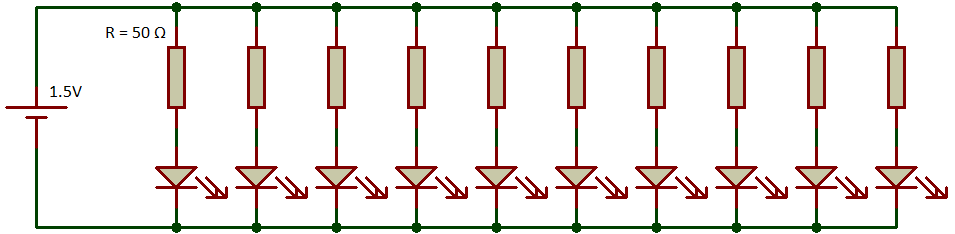
\includegraphics[width=13cm]{assets/figures/schema_leds1.png}
    \caption{Eclairage de test - Schéma électrique de la rangée de led - Schéma modifié de: \url{https://www.sonelec-musique.com/electronique_realisations_alim_led.html}}
\end{figure}
Les veroboards sont pratiques à manipuler, il est possible se les tenir avec des étaux afin de faire varier les positions durant les tests. Une fois monté,
le résultat est le suivant:
\begin{figure}[H]
    \centering
    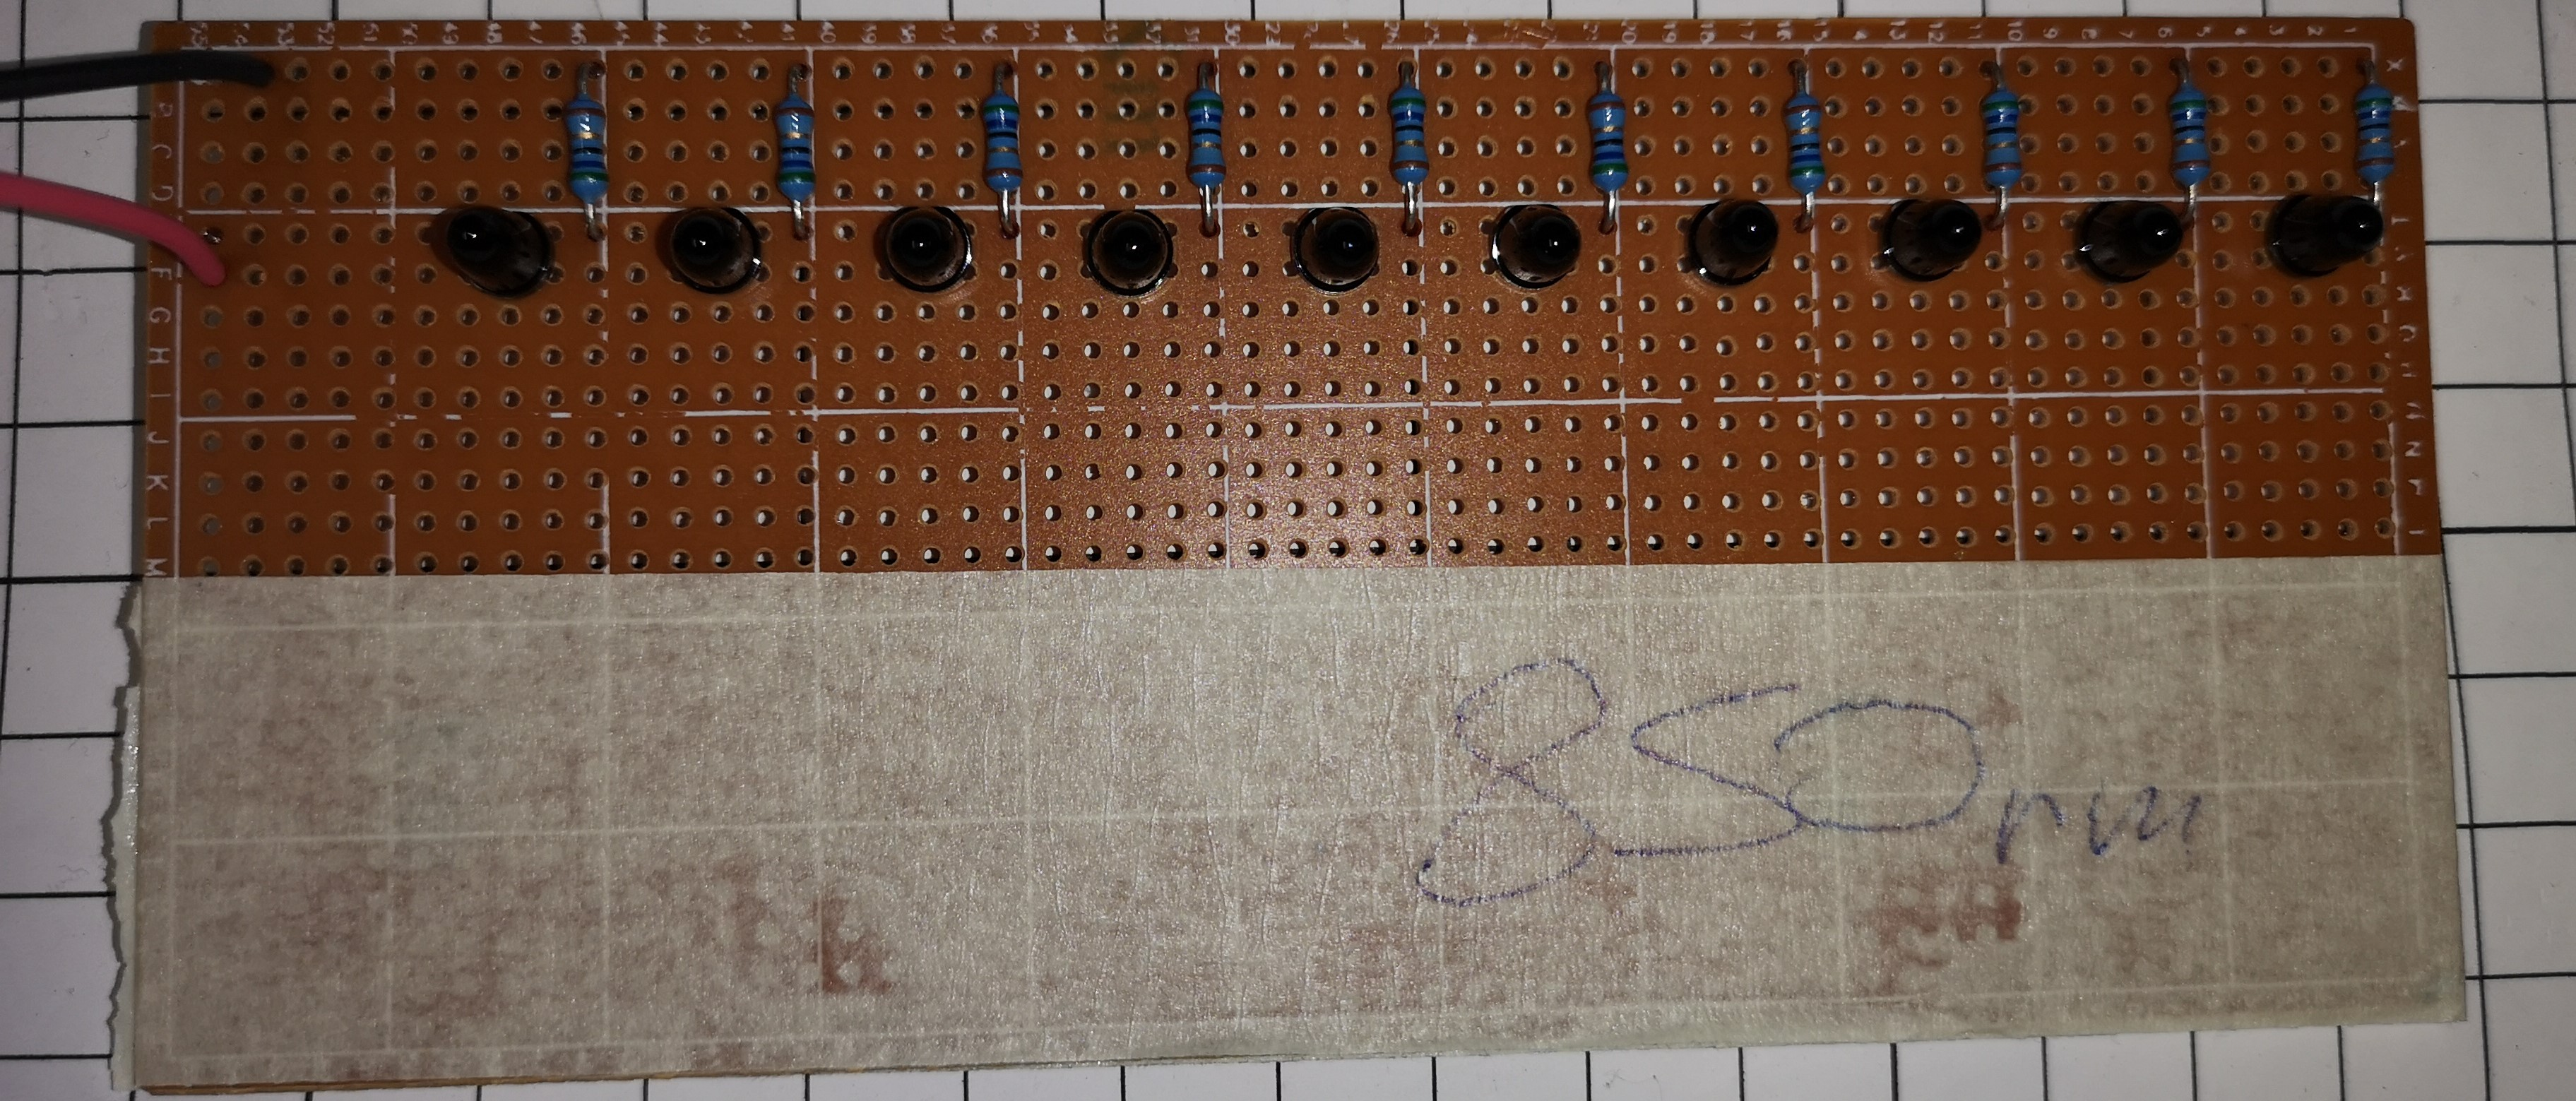
\includegraphics[width=10cm]{assets/figures/rail_led1.jpg}
    \caption{Eclairage de test - Rail de leds 1}
\end{figure}

\begin{figure}[H]
    \centering
    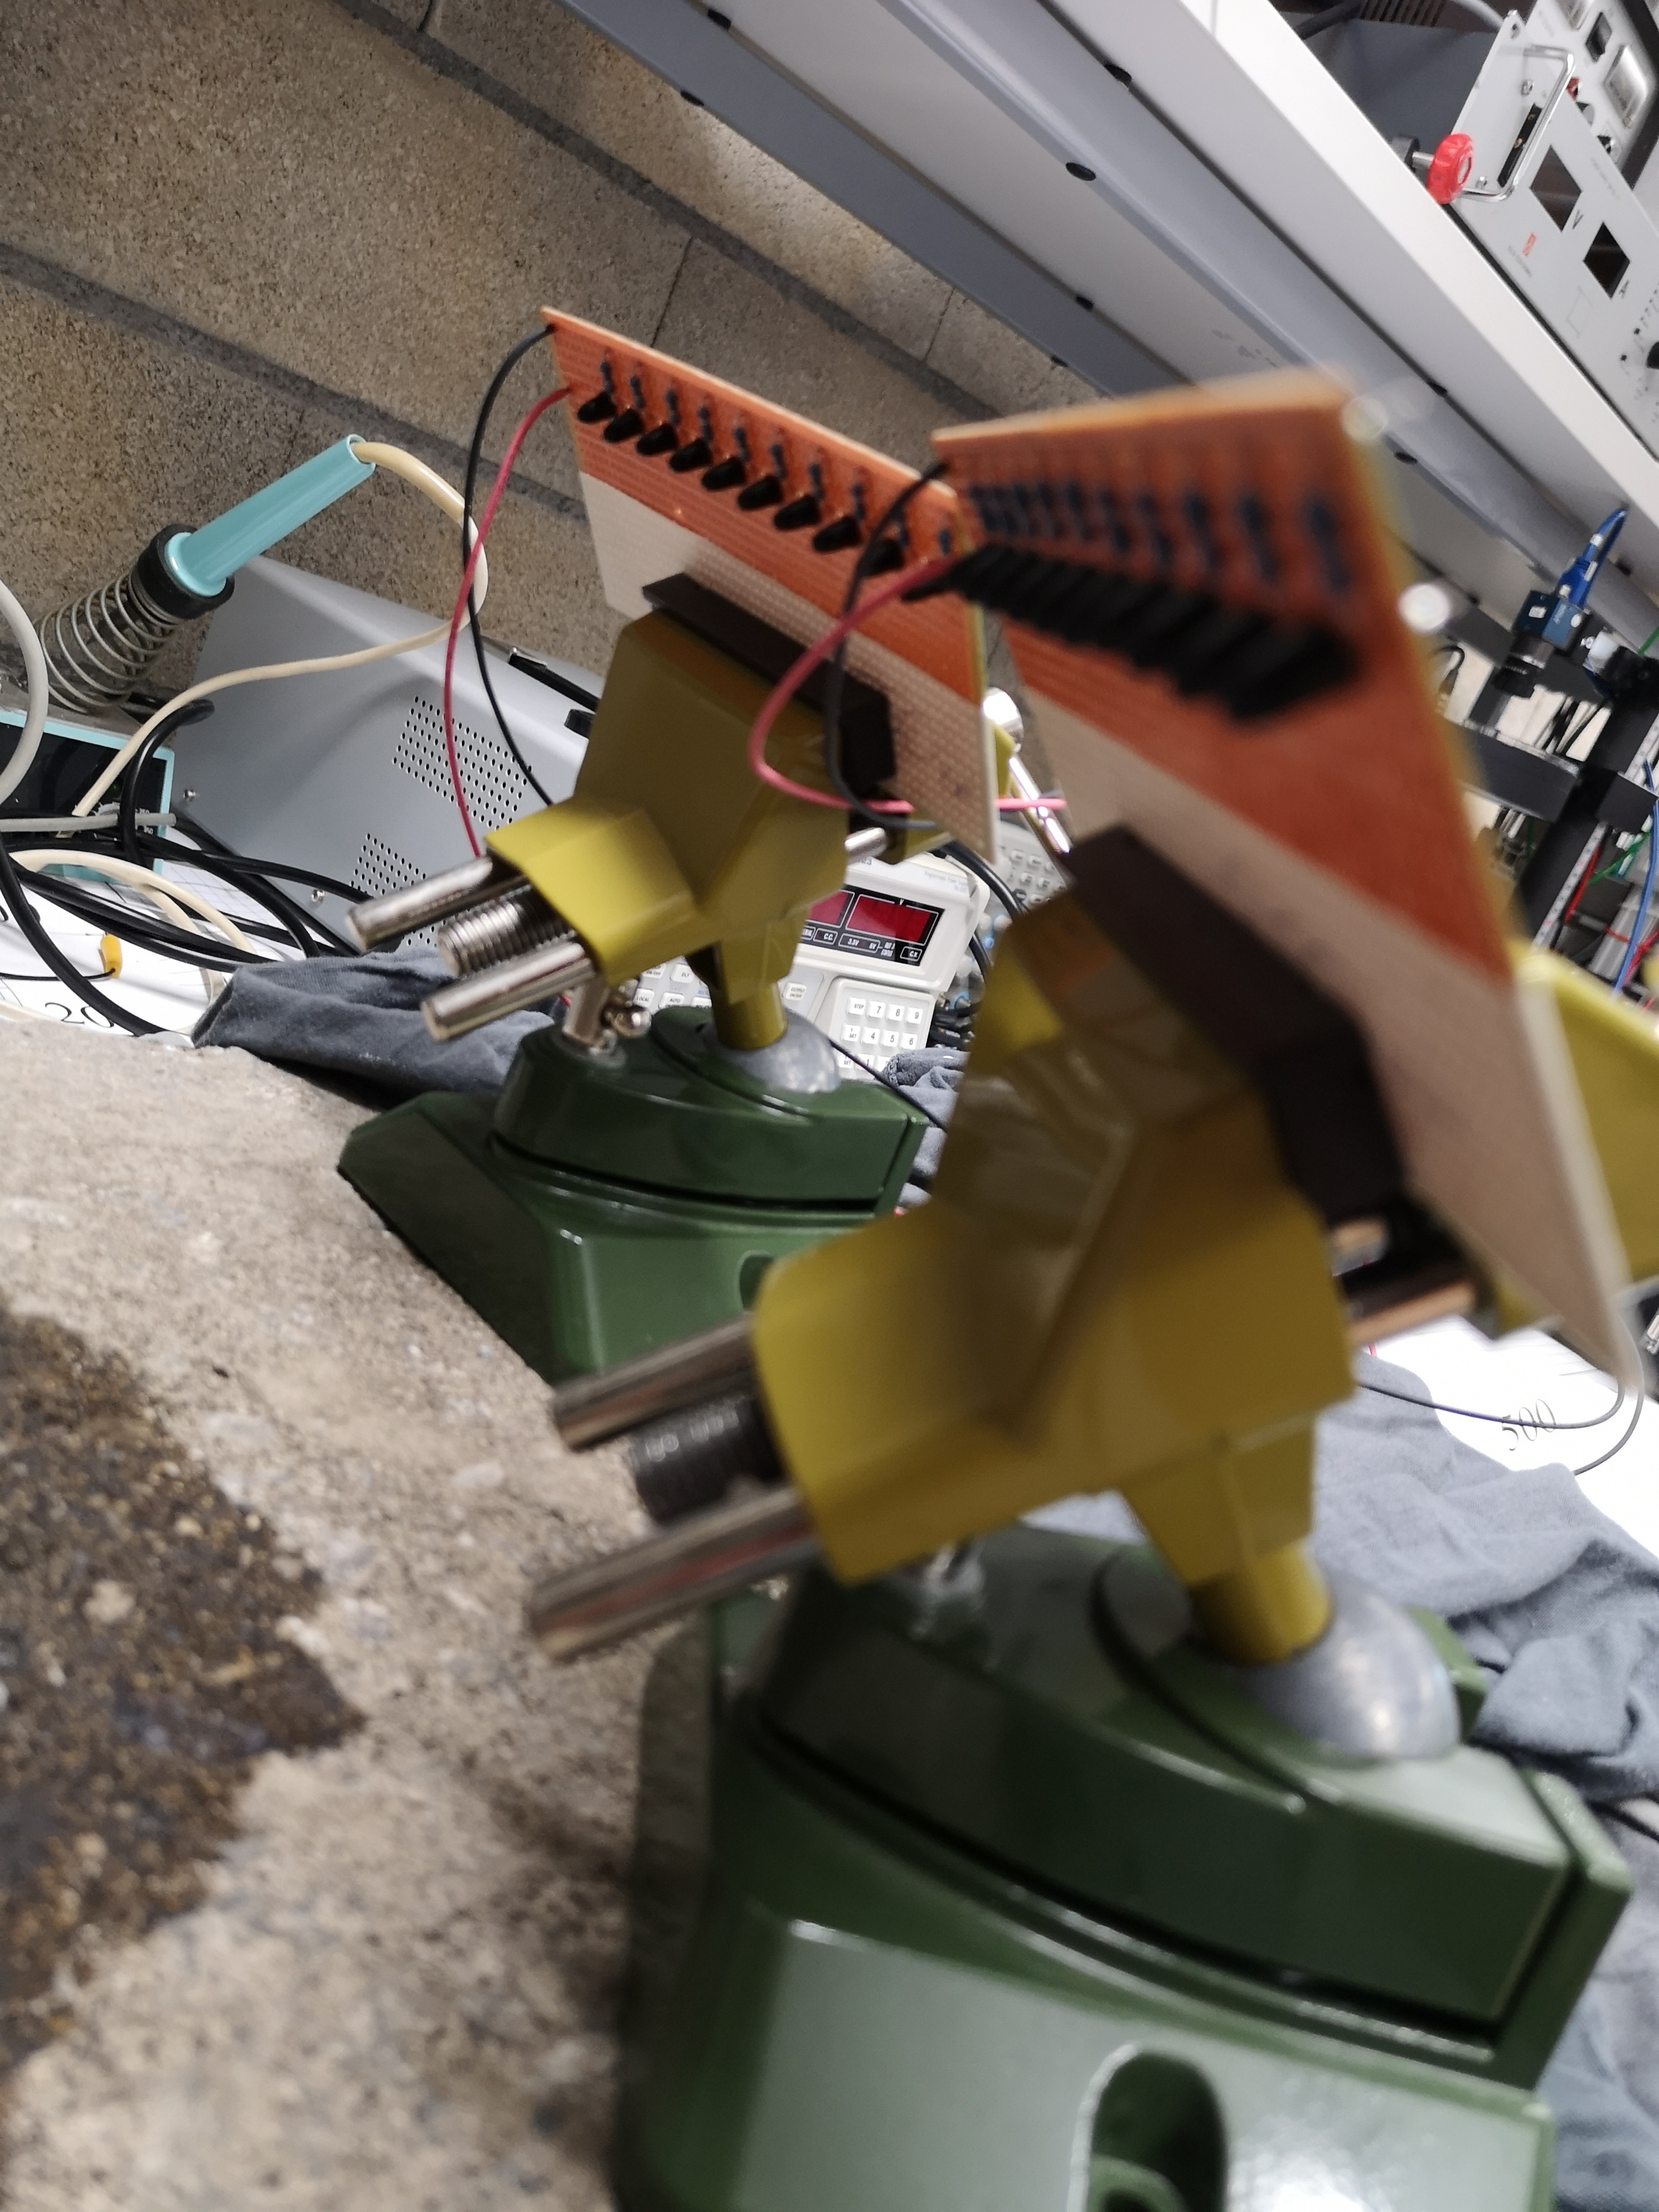
\includegraphics[width=6cm]{assets/figures/rail_led2.jpg}
    \caption{Eclairage de test - Rail de leds 2}
\end{figure}
\subsection{Capture}
La capture d'acquisition des images de tests préliminaires se fait via la caméra sélectionnée durant la phase de décision, un Rpi4 ainsi
qu'un petit script configurant la caméra et enregistrant l'image. (Script en annexe \ref{test_process})
\newpage
\subsection{Images}
Vu depuis la caméra, nous avons la scène suivante:

\begin{figure}[H]
    \centering
    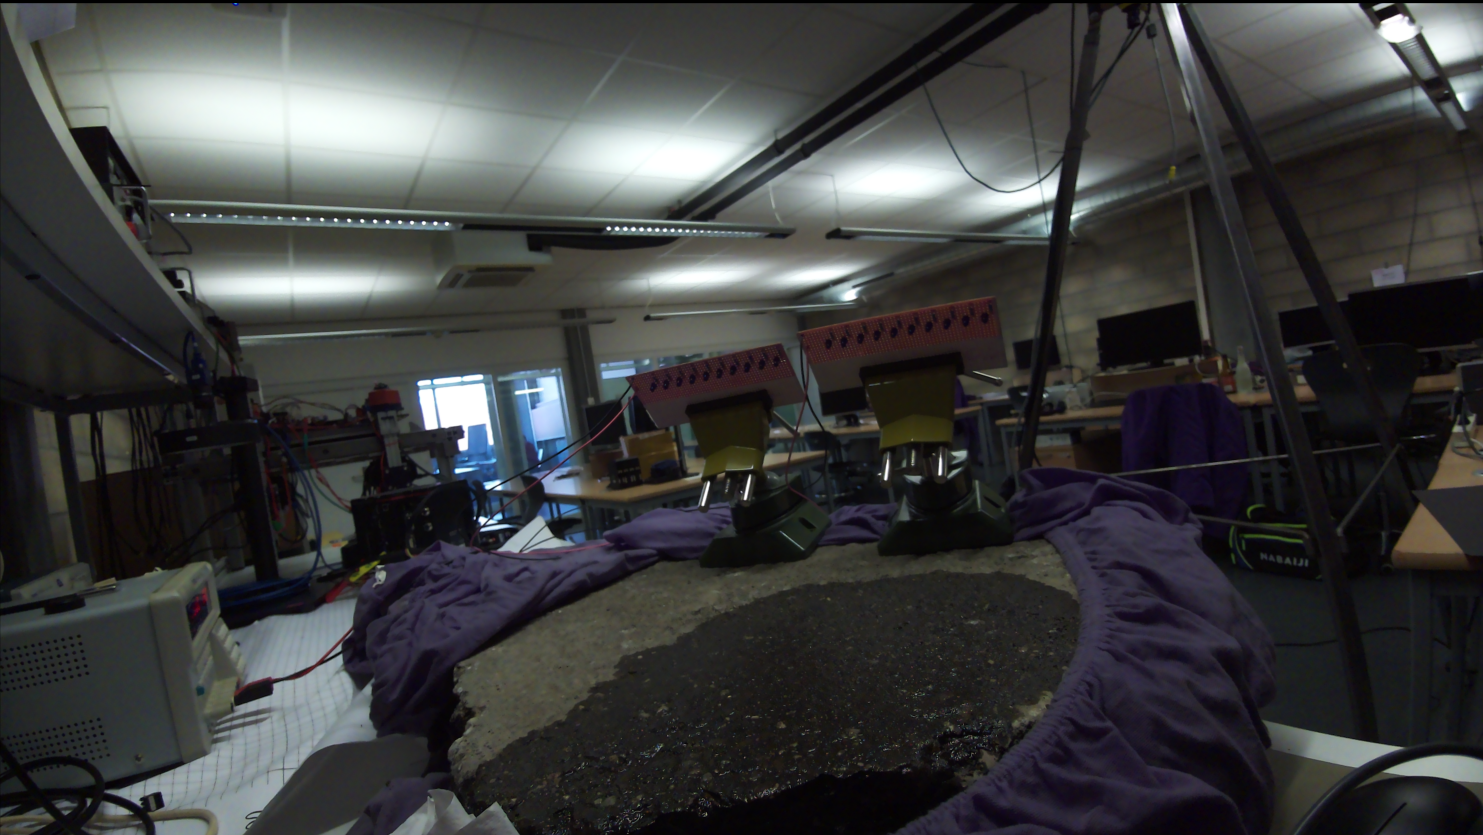
\includegraphics[width=13cm]{assets/figures/camera_vue_couleur1.png}
    \caption{Capture de test - Vue de la scène en couleur}
\end{figure}

Au moment d'effectuer les tests de sensibilités aux IR, tout le matériel n'était pas encore arrivé, notamment le filtre de l'objectif ne
laissant passer que les infrarouges. J'ai donc effectué les captures qui vont suivre dans les conditions suivantes:
\begin{itemize}
    \item Lumières éteintes dans la pièce.
    \item Deux lignes de 10 leds IR éclairant en direction de la tâche d'huile de moteur.
    \item Protection contre les lumières parasites du couloir (carton).
    \item Auto-focus sur le centre de l'image
    \item Temps d'exposition: 5000[ns] (déterminé expérimentalement avec plusieurs captures).
\end{itemize}
Avec ce setup, j'ai effectué plusieurs captures en faisant varier la position de l'éclairage par rapport à la tâche d'huile et la caméra.
J'ai obtenu différents résultats, plus ou moins utilisables.


Ci-dessous, un exemple d'éclairage orienté "contre" la caméra selon la figure suivante:
\begin{figure}[H]
    \centering
    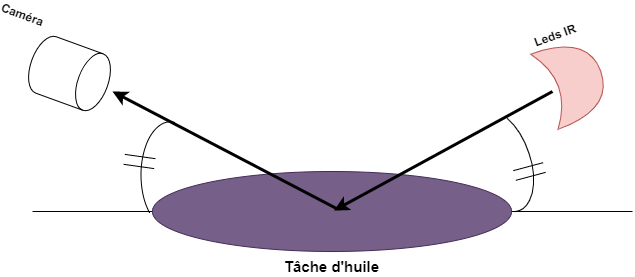
\includegraphics[width=13cm]{assets/figures/eclairage_contre_camera.png}
    \caption{Schéma de capture - Eclairage contre la camera \label{led_perp}}
\end{figure}


\begin{figure}[H]
    \centering
    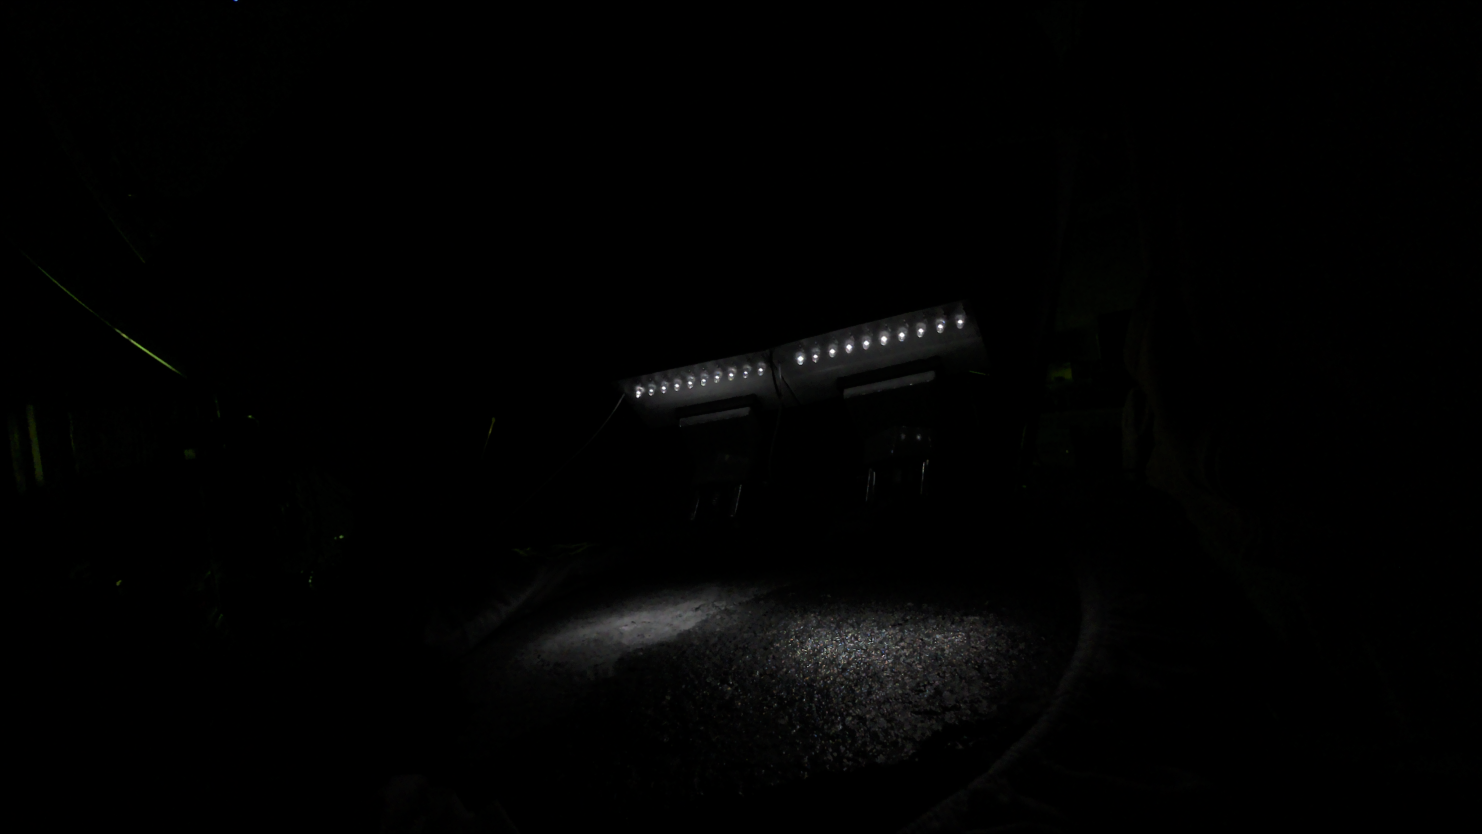
\includegraphics[width=13cm]{assets/figures/eclairage_face1.png}
    \caption{Capture de test - éclairage de face 1}
\end{figure}
\begin{figure}[H]
    \centering
    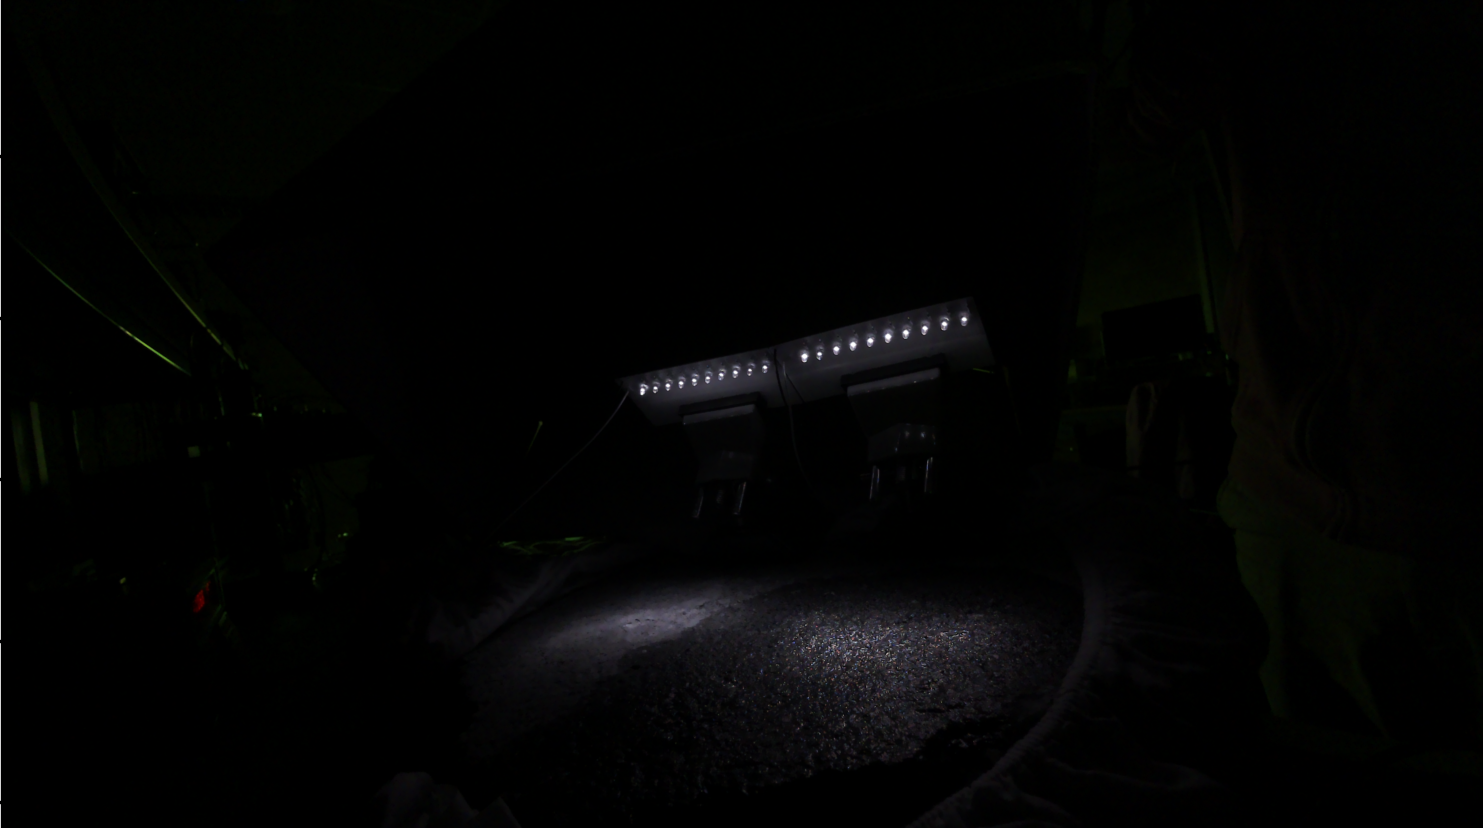
\includegraphics[width=13cm]{assets/figures/eclairage_face2.png}
    \caption{Capture de test - éclairage de face 2}
\end{figure}

On observe que la route et l'huile reflètent les leds IR, à l'oeil nu la différence est notable, mais l'analyse avec un soft peut s'avérer compliquée.

Ci-dessous, un exemple d'éclairage orienté perpendiculairement à la route selon la figure suivante:
\begin{figure}[H]
    \centering
    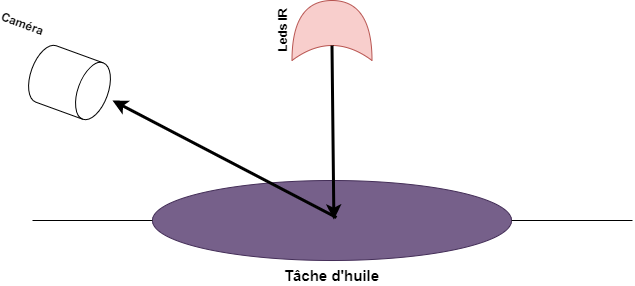
\includegraphics[width=13cm]{assets/figures/eclairage_perpendiculaire.png}
    \caption{Schéma de capture - Eclairage perpendiculaire à la route}
\end{figure}

\begin{figure}[H]
    \centering
    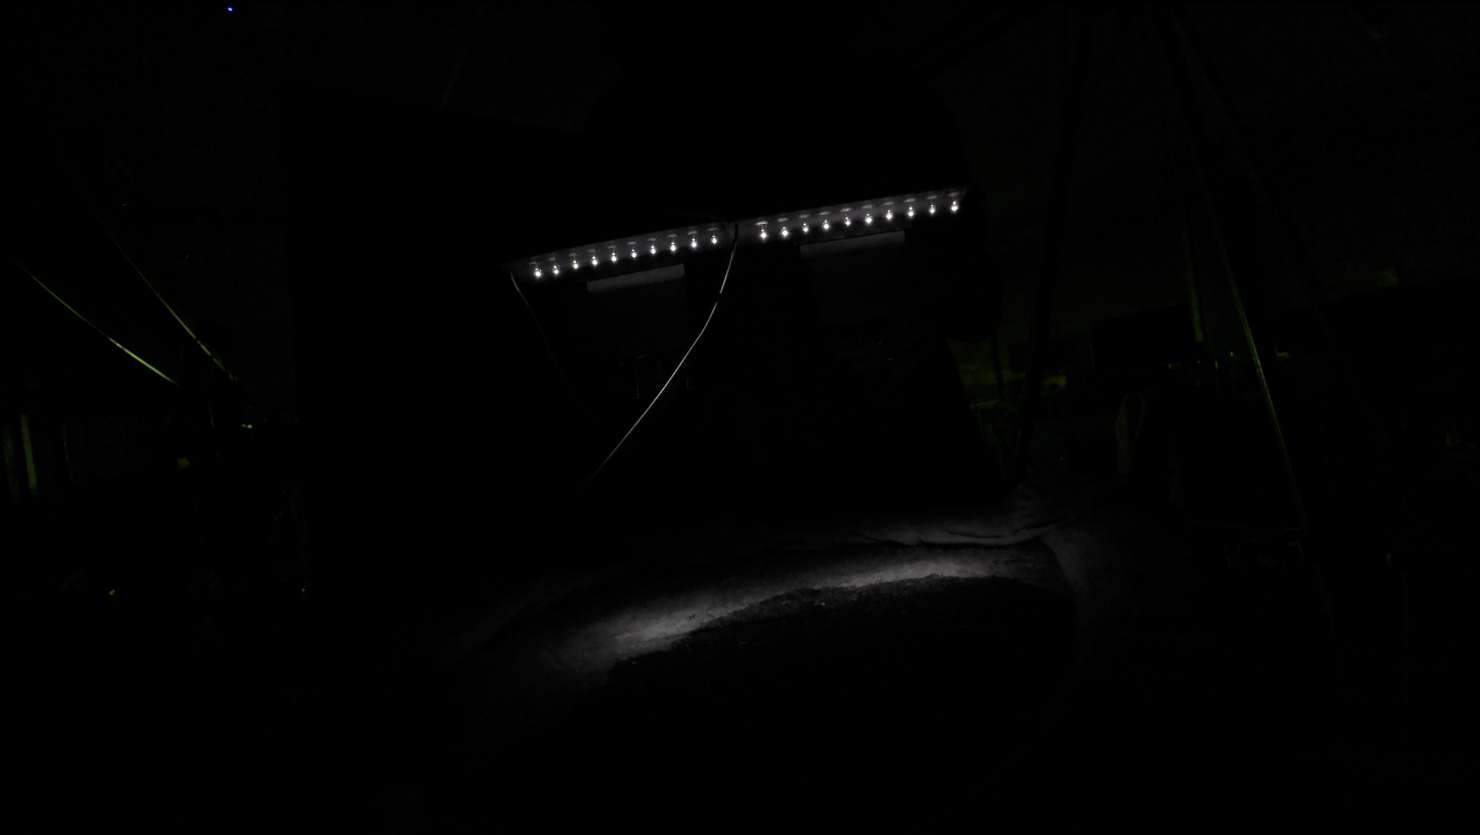
\includegraphics[width=13cm]{assets/figures/eclairage_perpendiculaire1.png}
    \caption{Capture de test - Eclairage perpendiculaire 1}
\end{figure}
\newpage
\begin{figure}[H]
    \centering
    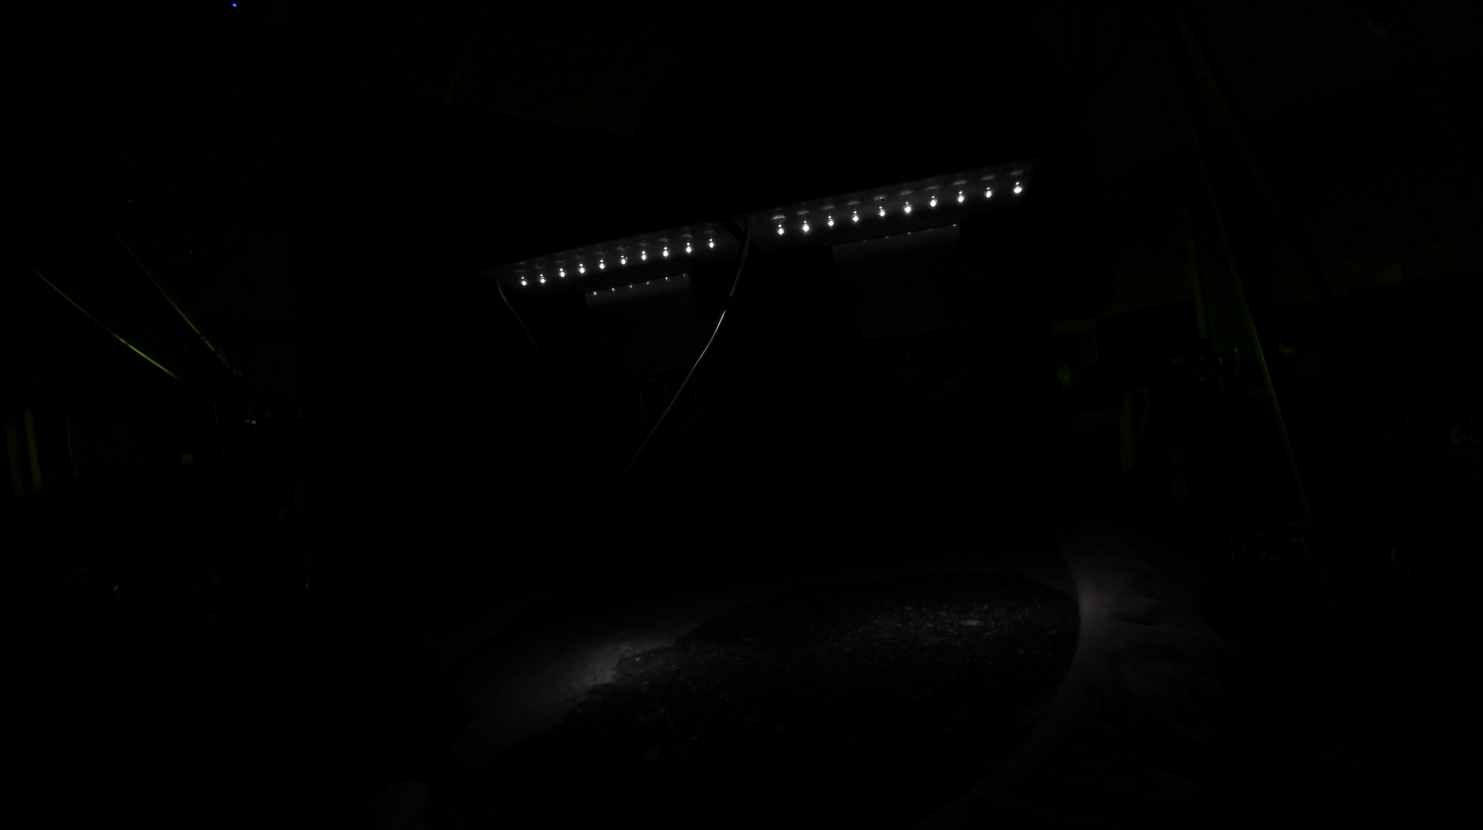
\includegraphics[width=13cm]{assets/figures/eclairage_perpendiculaire2.png}
    \caption{Capture de test - Eclairage perpendiculaire 2}
\end{figure}

\begin{figure}[H]
    \centering
    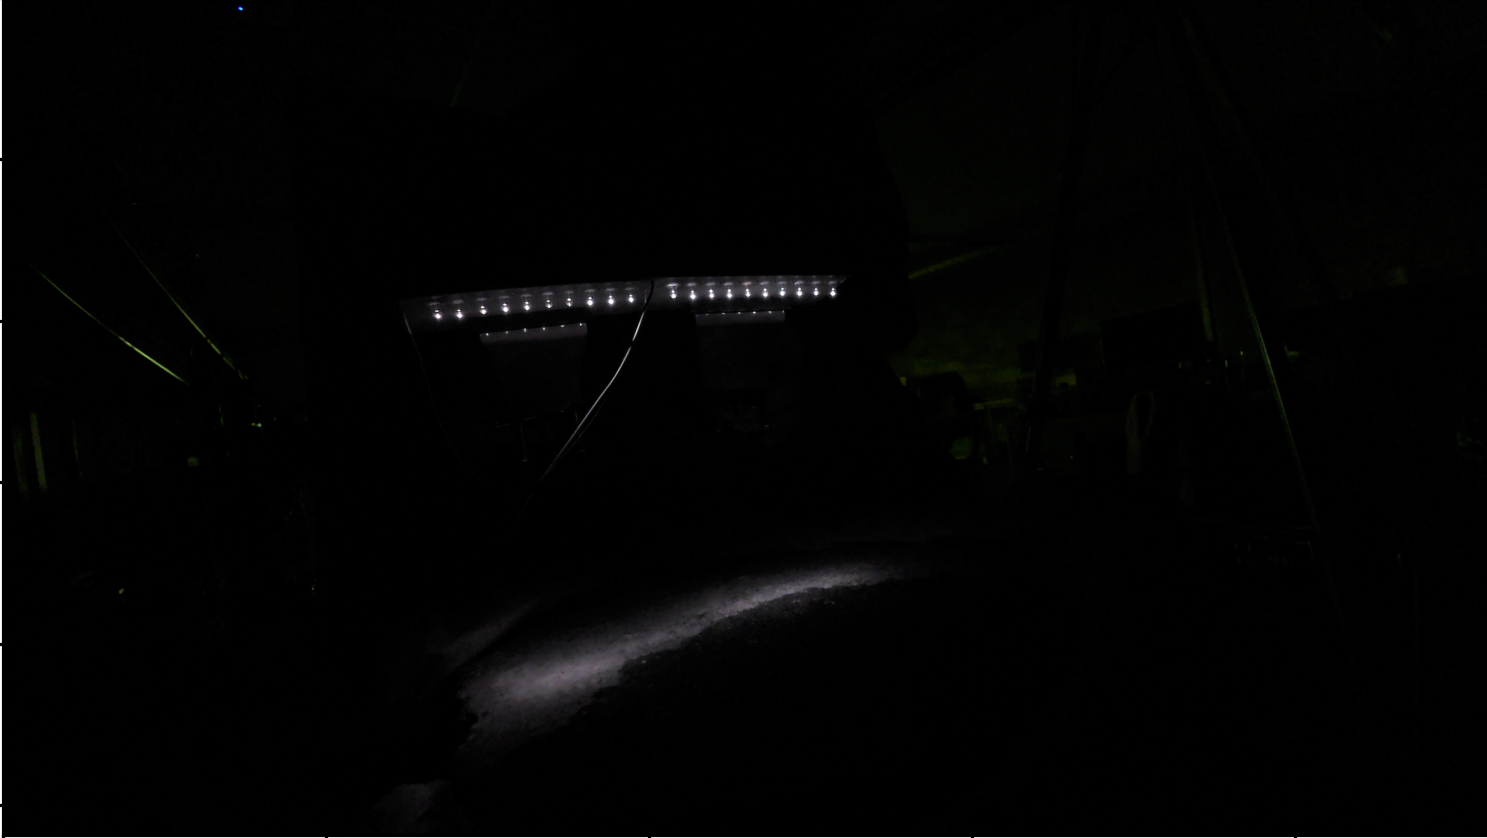
\includegraphics[width=13cm]{assets/figures/eclairage_perpendiculaire3.png}
    \caption{Capture de test - Eclairage perpendiculaire 3}
\end{figure}
\newpage
On observe que la route diffuse, dans une moindre mesure, l'éclairage des leds IR, là où l'huile semble absorber les rayonnements. On arrive
assez facilement à différencier le clair de la route et le foncé de l'huile. La mise en place d'un software de détection est envisageable avec
un éclairage basé sur ce schéma. A noter que les tests ont été effectués avec plusieurs gammes de leds (830nm, 850nm et 880nm), la différence
sur le retour image n'est pas très grandes, mais les leds 850nm permettent de mieux différencier la route de l'huile.

La visibilité des captures présentées sont peut-être de moins bonne qualité sur la version papier du rapport.

J'ai également tenté la configuration suivante:
\begin{figure}[H]
    \centering
    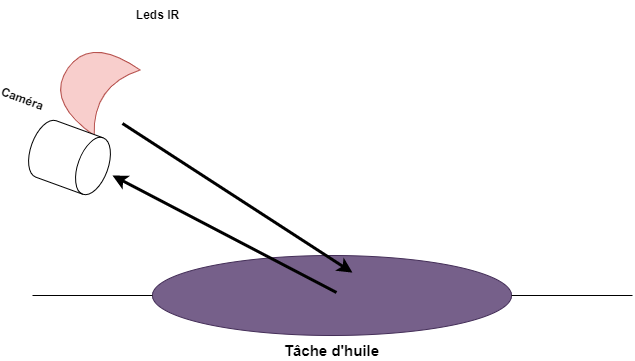
\includegraphics[width=13cm]{assets/figures/eclairage_dos.png}
    \caption{Schéma de capture - Eclairage de dos}
\end{figure}
Mais, étant trop sombre, les images obtenues n'étaient pas utilisables.
\newpage
\subsection{Filtre du visible}
J'ai effectué quelques tests supplémentaires après la réception des filtres ne laissant passer que l'infrarouge. Pour rappel, le filtre
ne laisse passer que les ondes supérieures à 700nm, les rouges lointains seront encore visibles.

Ci-dessous l'installation du matériel pour les captures de test:
\begin{figure}[H]
    \centering
    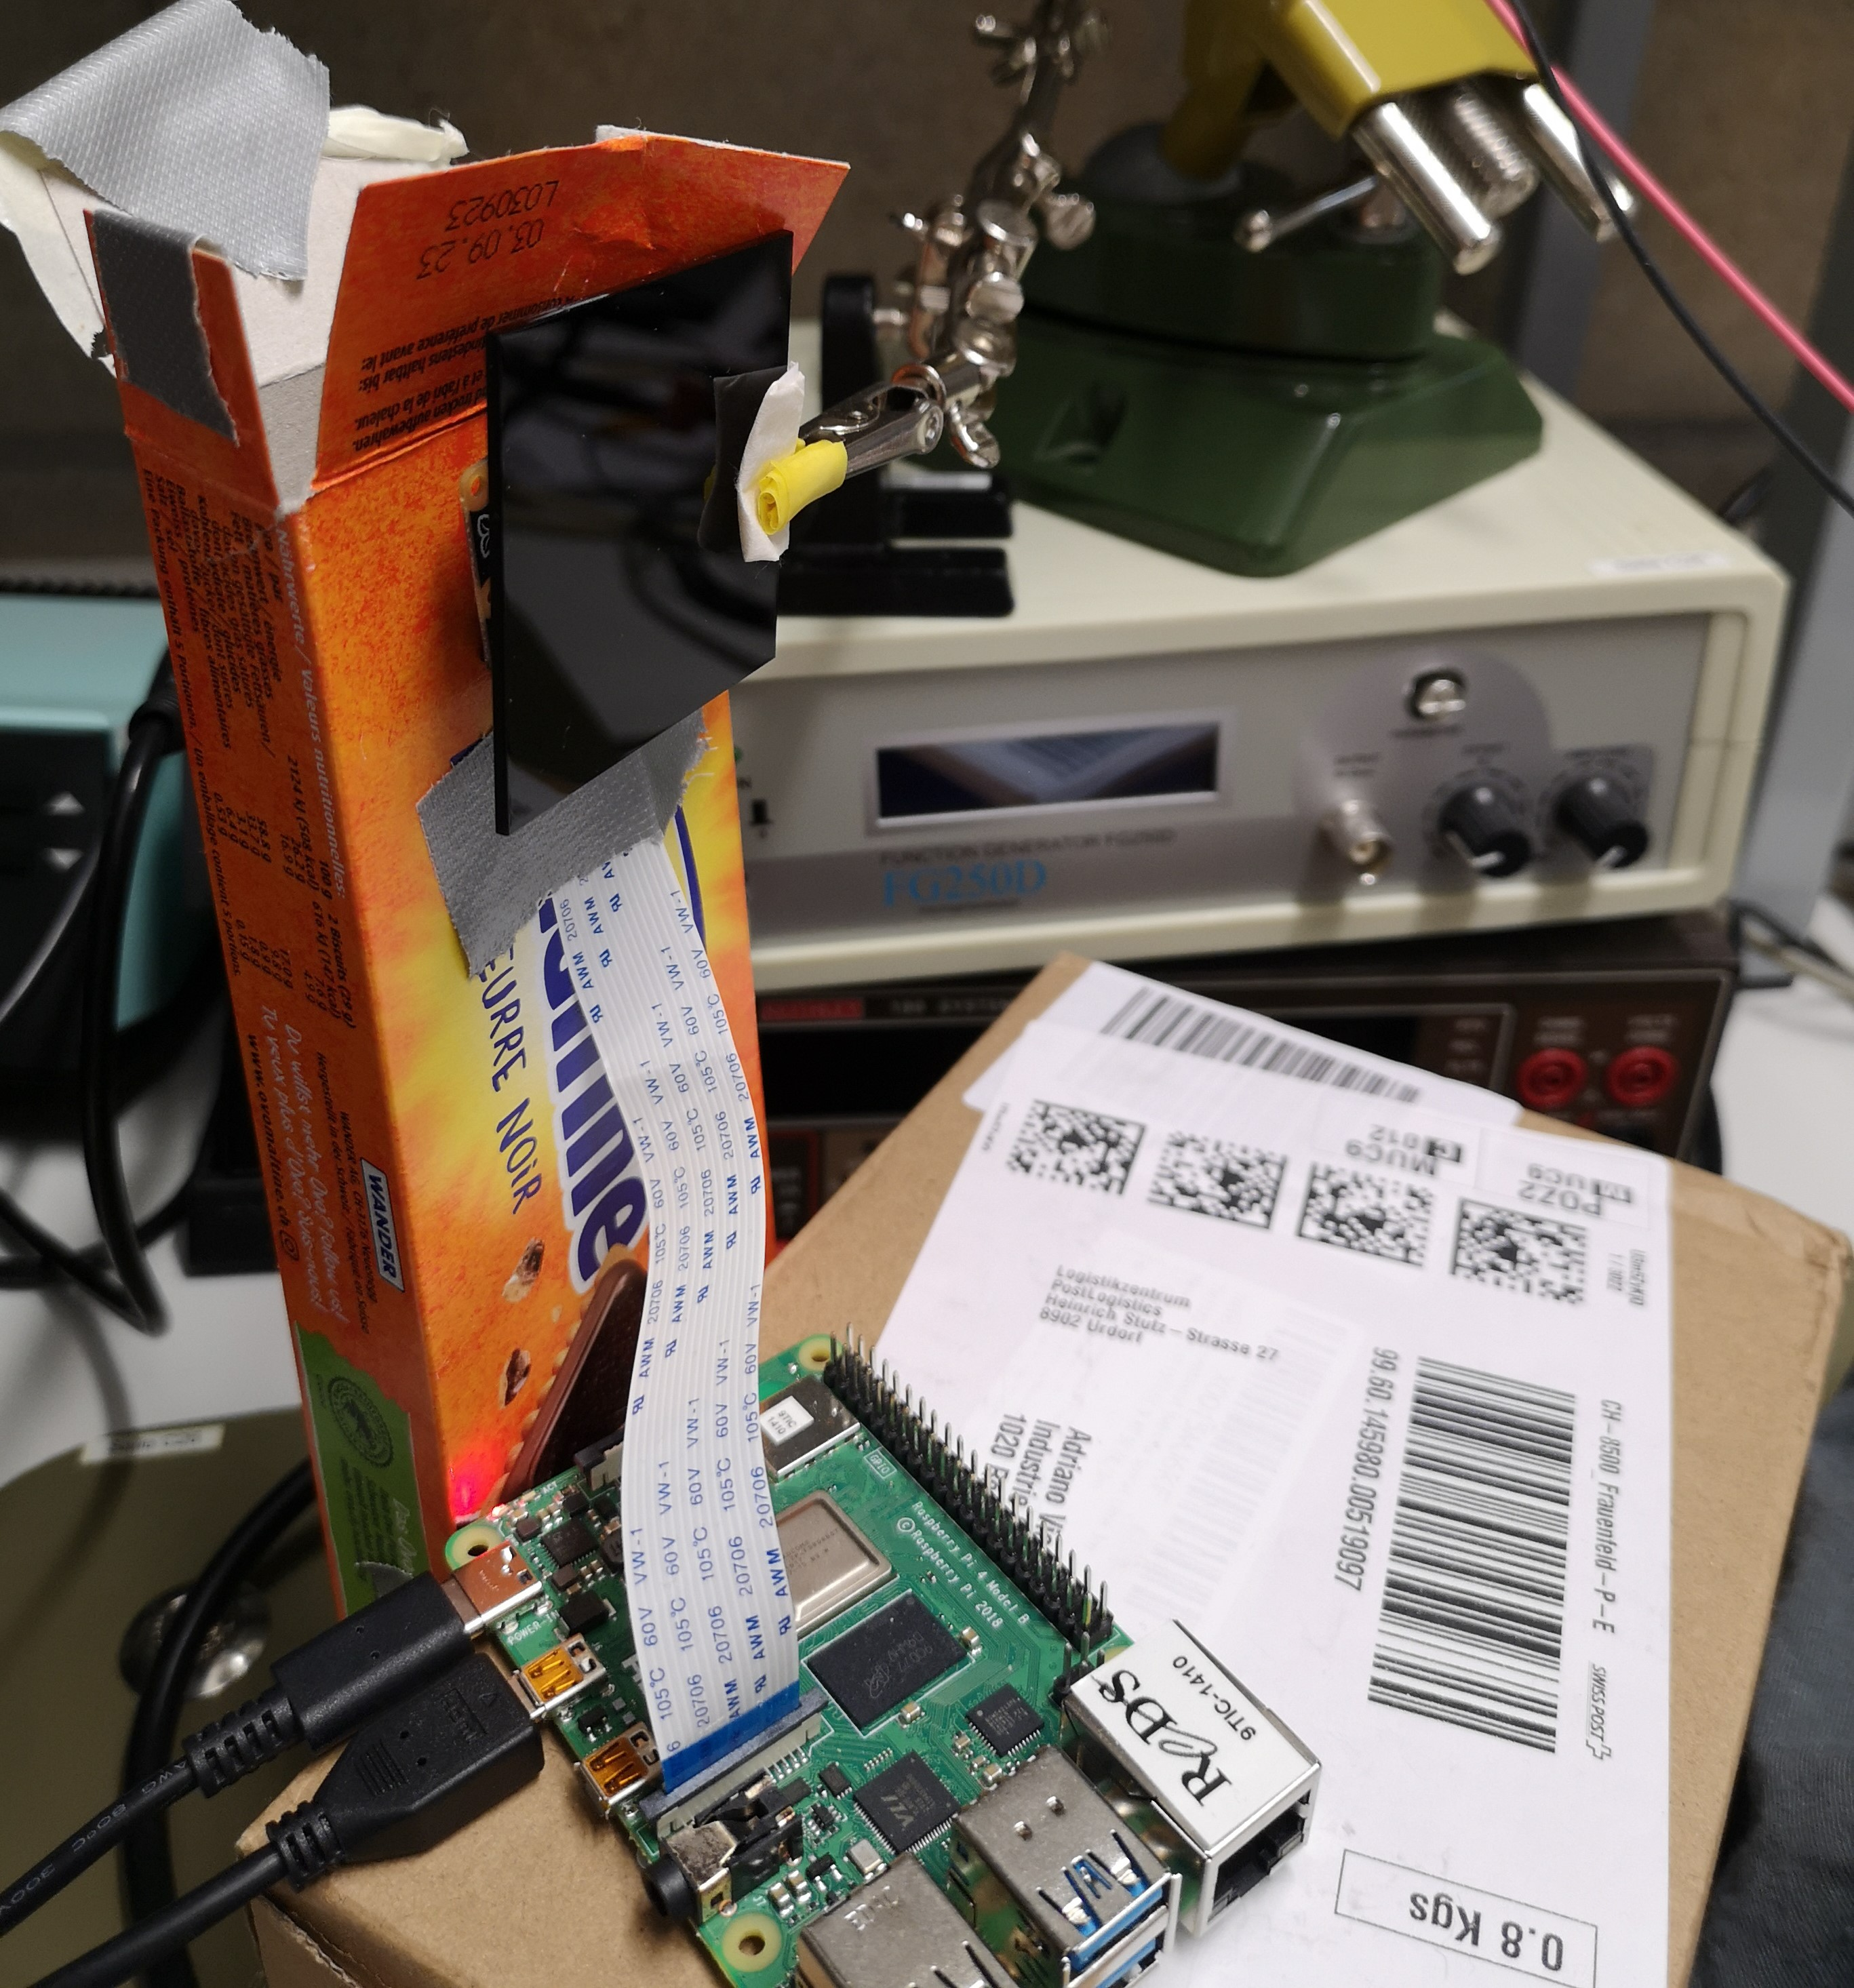
\includegraphics[height=11cm]{assets/figures/filtre.jpg}
    \caption{Capture avec filtre - Installation}
\end{figure}

Pour constater l'efficacité du filtre, j'ai effectué 3 captures.
\begin{itemize}
    \item Une image simple.
    \item Une image avec l'éclairage IR enclenché.
    \item Une image avec l'éclairage IR enclenché selon la figure \ref{led_perp}.
\end{itemize}
On notera également que le filtre perturbe l'autofocus du capteur, la position de la lentille a donc été définie en dur dans le code de test.
Les informations concernant ces réglages se trouvent au chapitre 5.2.3 de la documentation Picamera2 \cite{picamera2}.

\begin{figure}[H]
    \centering
    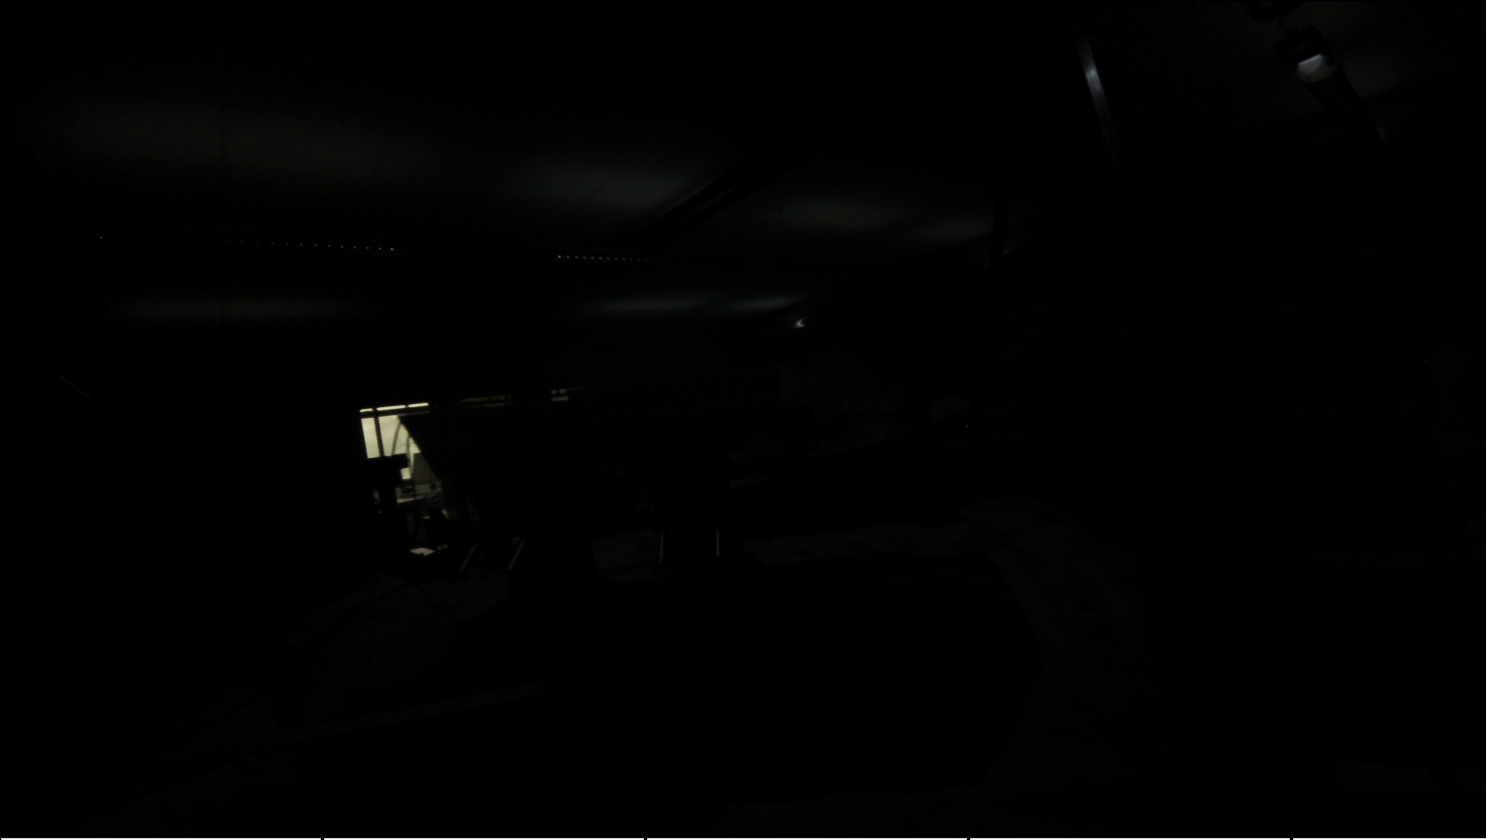
\includegraphics[width=13cm]{assets/figures/filtre_simple.png}
    \caption{Capture avec filtre - Environnement simple}
\end{figure}
\begin{figure}[H]
    \centering
    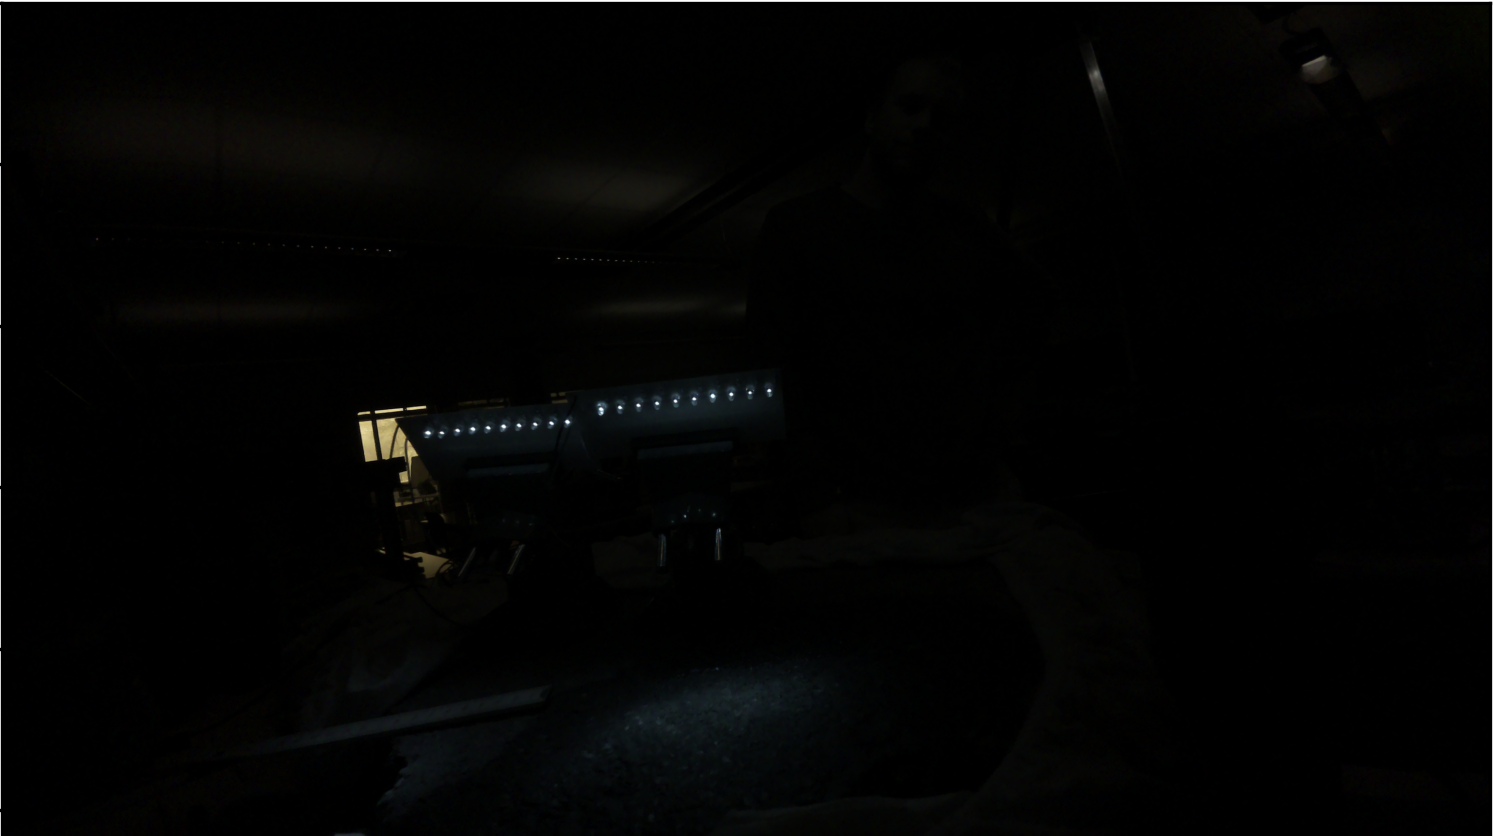
\includegraphics[width=13cm]{assets/figures/filtre_IR.png}
    \caption{Capture avec filtre - Leds IR allumées}
\end{figure}
\newpage
\begin{figure}[H]
    \centering
    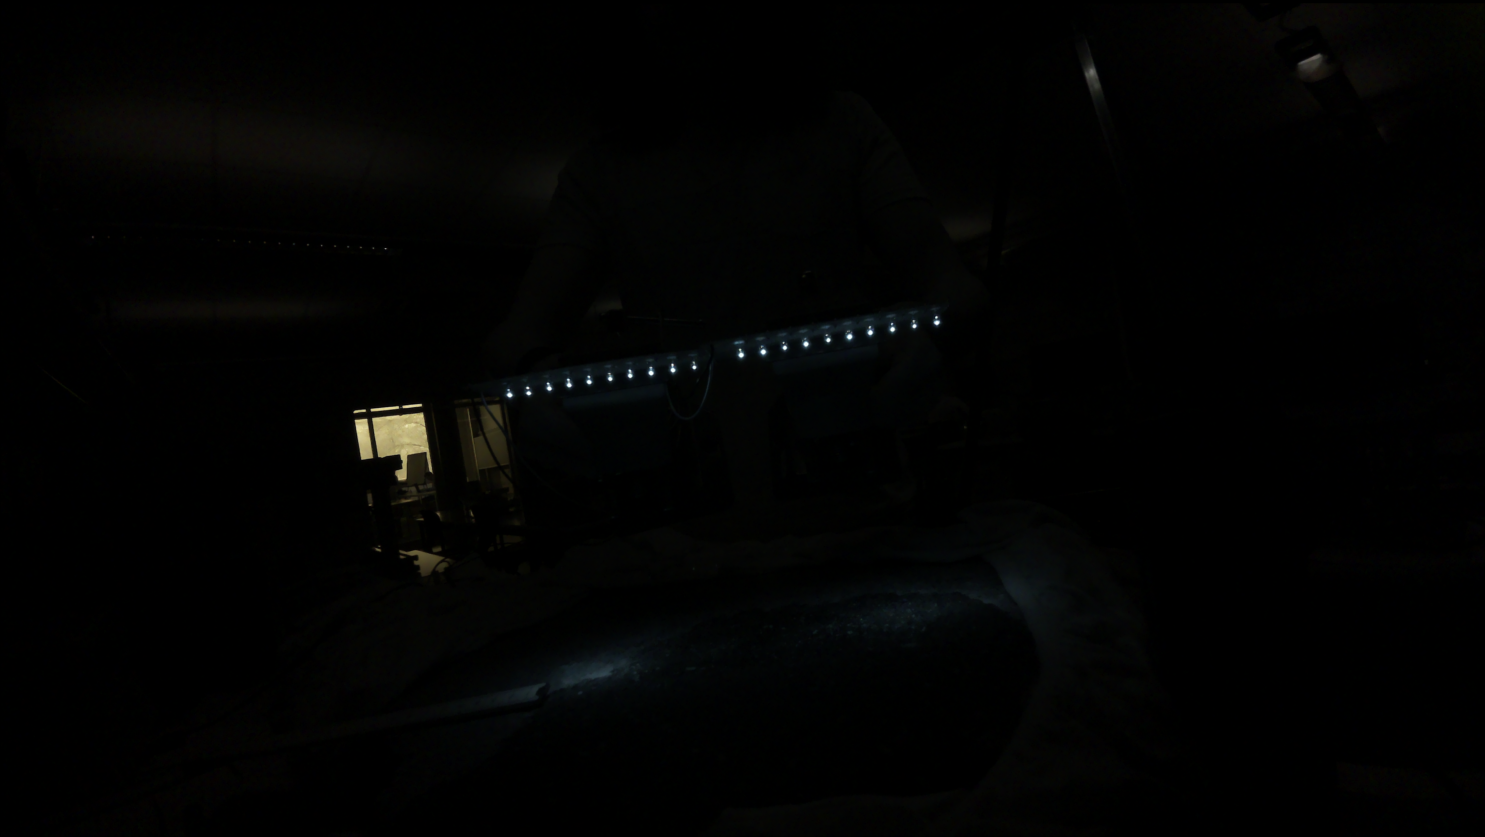
\includegraphics[width=13cm]{assets/figures/filtre_IR_huile.png}
    \caption{Capture avec filtre - Leds IR selon figure \ref{led_perp}}
\end{figure}
On observe que la quasi totalité des éclairages de la pièce disparaissent de la capture,
mettant en évidence la route et la trace d'huile au milieu de celle-ci. Il reste cependant les rayonnements solaires (visible sur la partie gauche des images)
à gérer, le soleil émettant dans un large spectre, ceux-ci apparaissent dans l'image. L'emplacement du laboratoire ne permet pas de
tester le filtre et le capteur sous un ensoleillement tel qu'on pourrait avoir en extérieur, précédemment il a été démontrer que l'emplacement
de l'éclairage par rapport aux traces influait sur la qualité de la capture, il doit en être de même concernant l'emplacement du soleil. Des tests dans
différentes conditions doivent être effectués.

\section{Installation}
\subsection{Eclairage}
Le but est de garder le même principe d'éclairage que durant les tests préliminaires, c'est à dire un éclairage perpendiculaire au sol,
en bande, avec des leds IR émettant à 850nm. De plus, il faudrait dans l'idéal que le système d'éclairage suive les contraintes suivantes:
\begin{itemize}
    \item Diffusion en bande.
    \item Largeur de 150cm.
    \item Possiblement repliable si non utilisés.
    \item Protégé pendant les déplacements.
\end{itemize}
J'envisage de fabriquer le rails de leds sur les principes suivants:
\begin{enumerate}
    \item Elément solide sur lequel braser les leds (veroboard).
    \item Structure solide sur lequel fixer les veroboards (profilé plat).
    \item Tube de protection à enfiler lors des transports.
\end{enumerate}
\subsubsection{Veroboard}
La plaque de veroboard sert de conducteur permettant aux leds d'être alimentées. L'objectif est d'avoir deux bandes de leds de 75cm de part et d'autre
du timon. Je n'ai pas trouvé de veroboard faisant cette largeur, j'ai donc décidé d'utiliser les plaques disponibles au FabLab de l'HEIG et d'en faire un assemblage.
Le but est de transformer 5 plaques de 6.6cm x 15cm en 10 plaques de 3.3cm x 15cm afin de couvrir la largeur requise avec un minimum d'épaisseur.
Chaque plaque serait reliée à la suivante via un connecteur afin de transmettre l'alimentation.

L'implantation sur veroboard se ferait selon le plan suivant:
\begin{figure}[H]
    \centering
    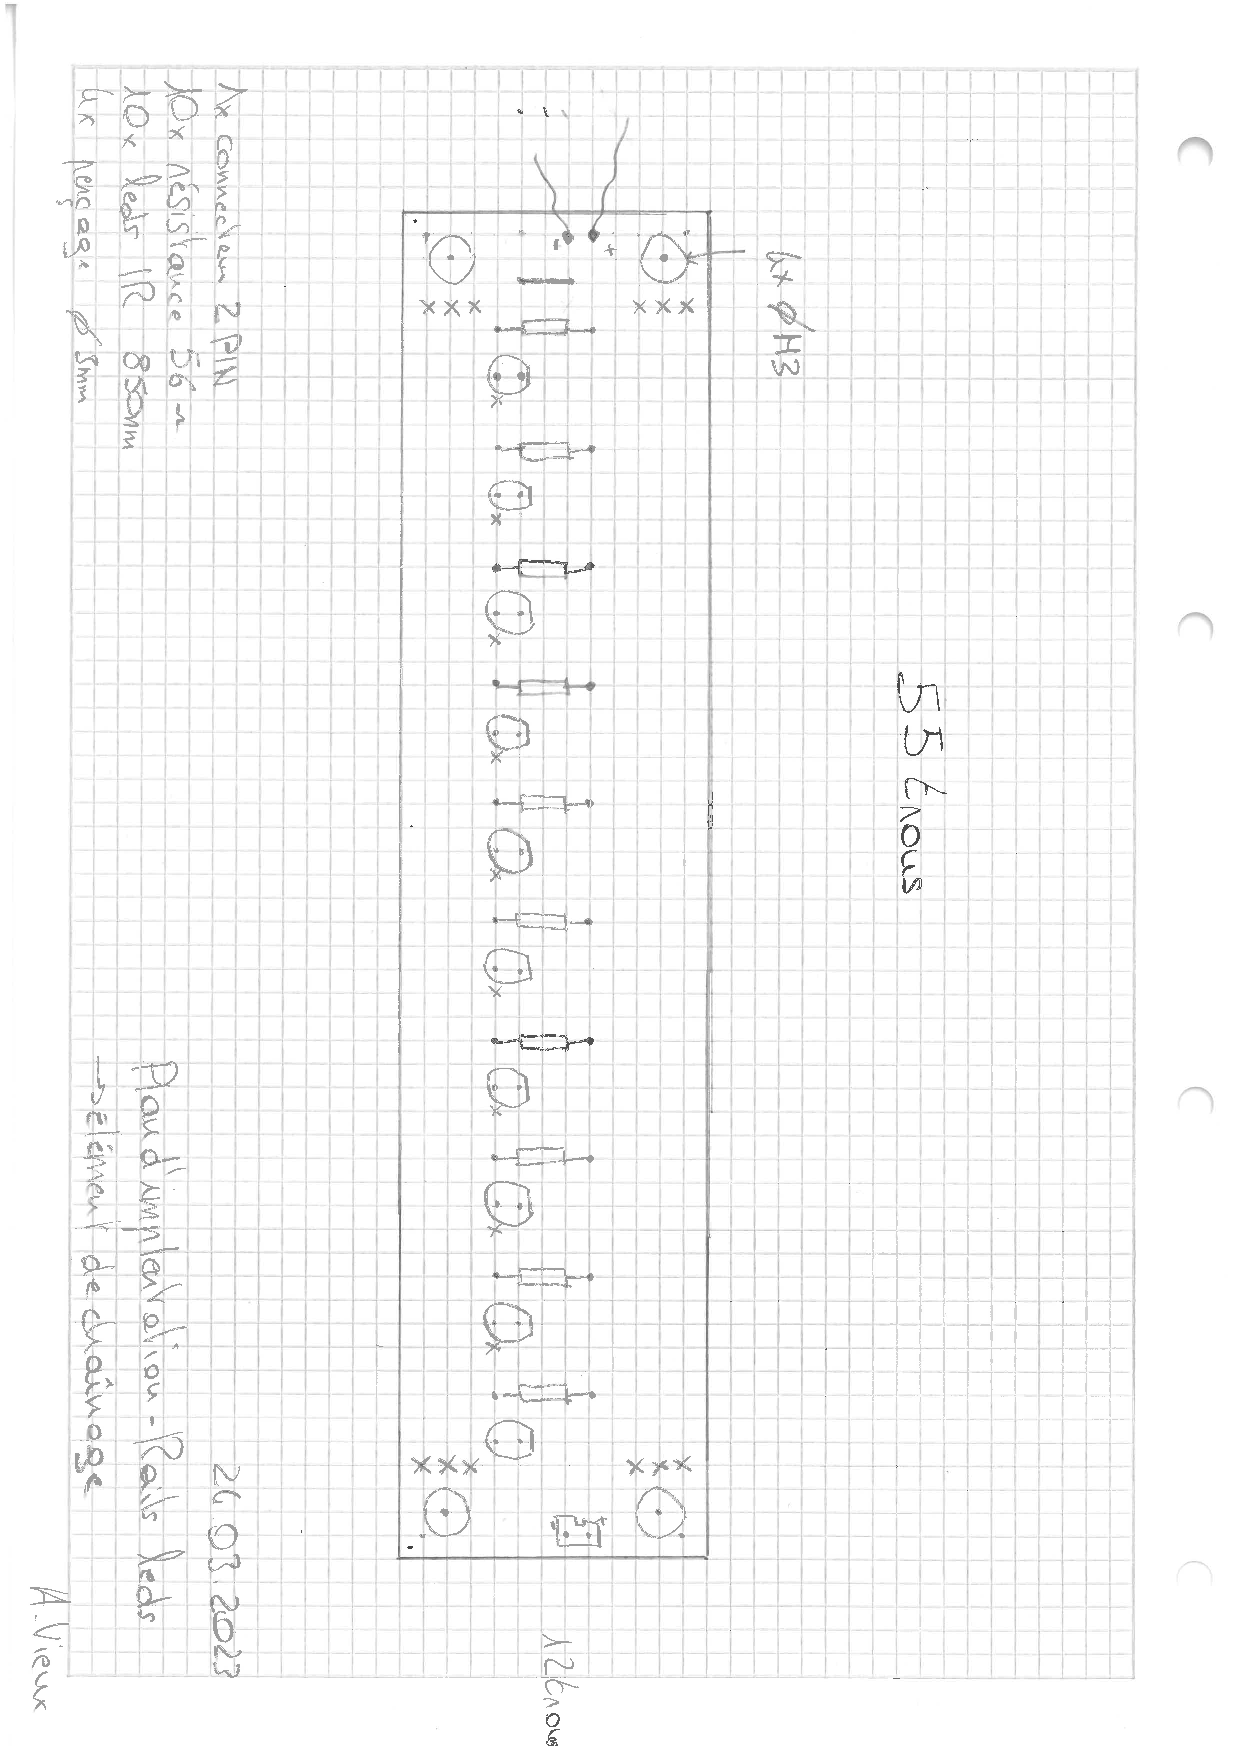
\includegraphics[width=10cm, trim=0 0 3cm 1cm, clip]{assets/figures/plan_implantation_rail_led.pdf}
    \caption{Plan d'implantation - Rail de Led}
\end{figure}

Notons que la chute de tension aux bornes des leds est de 1.3 V $\pm$ 0.1 V, celle-ci peut légèrement varier d'une led à l'autre. C'est
pourquoi il est important de mettre une résistance avant chaque led, de manière à ce que celle-ci gère le potentiel surplus de tension.
De plus, cela permet d'avoir un contrôle sur le courant traversant la led et donc sur l'intensité de l'éclairage. Durant les tests préliminaires,
le courant traversant les leds étaient de 3,5 \si{\milli\A}, l'intensité lumineuse était bonne, je décide donc de m'y tenir.

\begin{figure}[H]
    \centering
    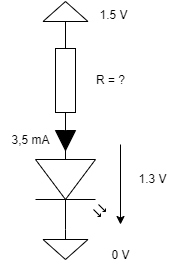
\includegraphics[height=7cm]{assets/figures/schema_led_res.png}
    \caption{Schéma électrique - Choix de résistance}
\end{figure}

Sachant \(R = U / I\), on se retrouve avec \(R = 0.2 / 0.0035 = 57.1 \si{\ohm} \) (Arrondi à 56\si{\ohm} dans la gamme de résistance E12).
\newpage
\subsubsection{Rails}
Les veroboards ont été placés sur deux profilés plats en aluminium percées et équipées d'entretoises de manières à accueillir le tout. Il suffit de poser les veroboards,
les fixer à l'aide de rondelles et boulons et de relier les alimentations d'une carte à l'autre. En cas de panne, le remplacement de la carte problématique est très rapide.

\begin{figure}[H]
    \centering
    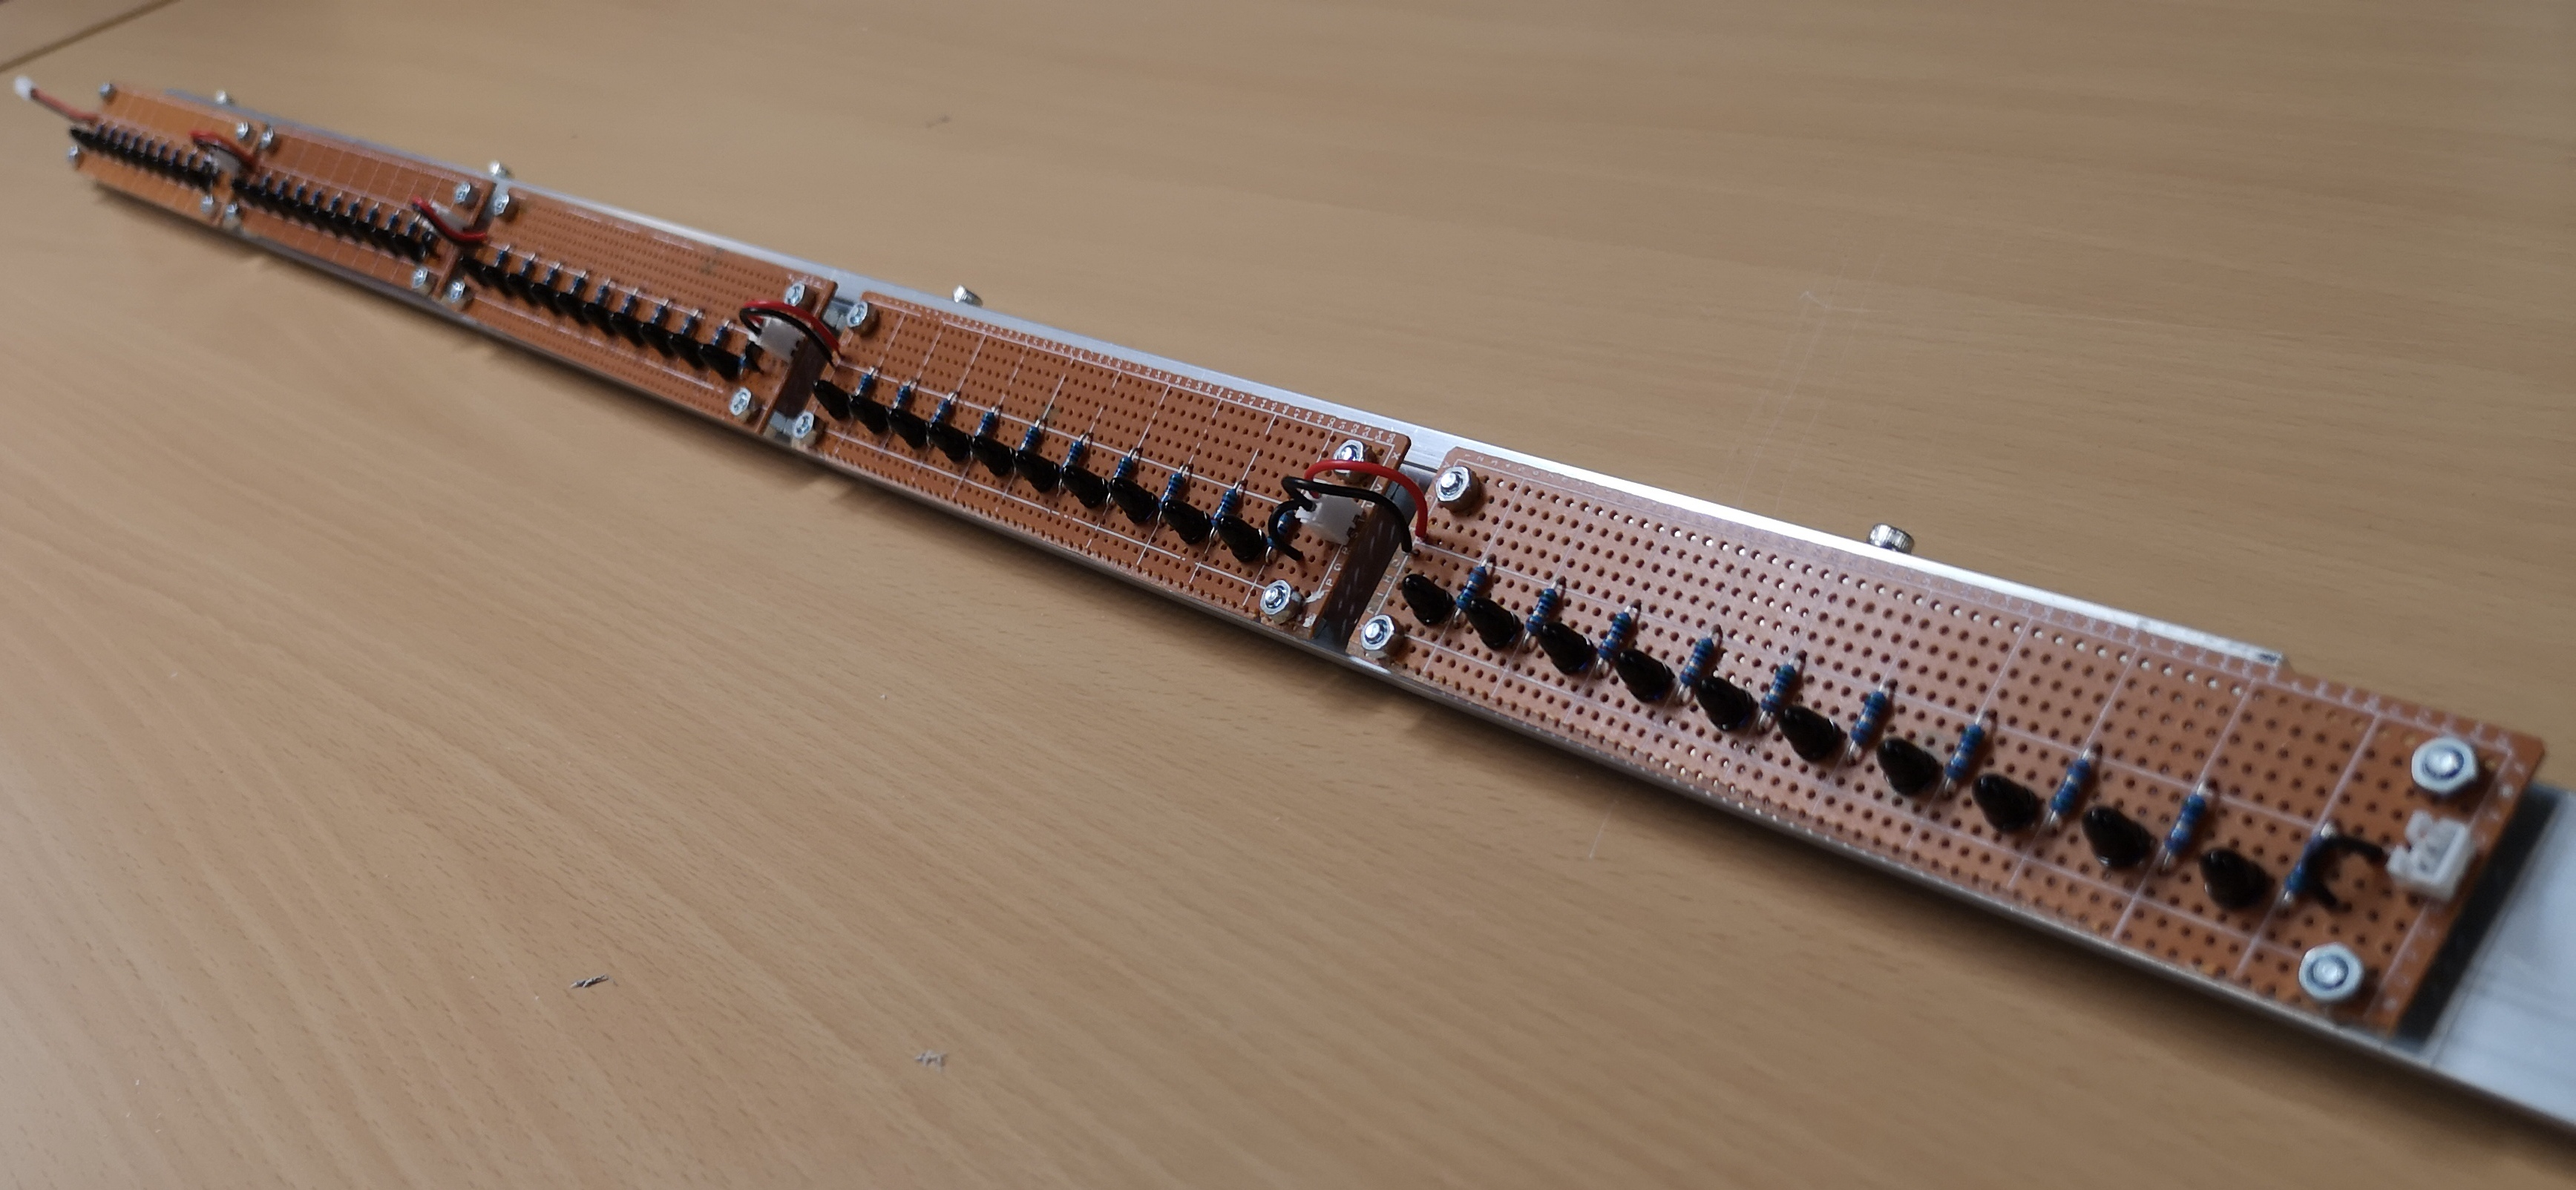
\includegraphics[height=7cm]{assets/figures/rail_alu_led.jpg}
    \caption{Assemblage - Rails leds sur profilé plat}
\end{figure}

\begin{figure}[H]
    \centering
    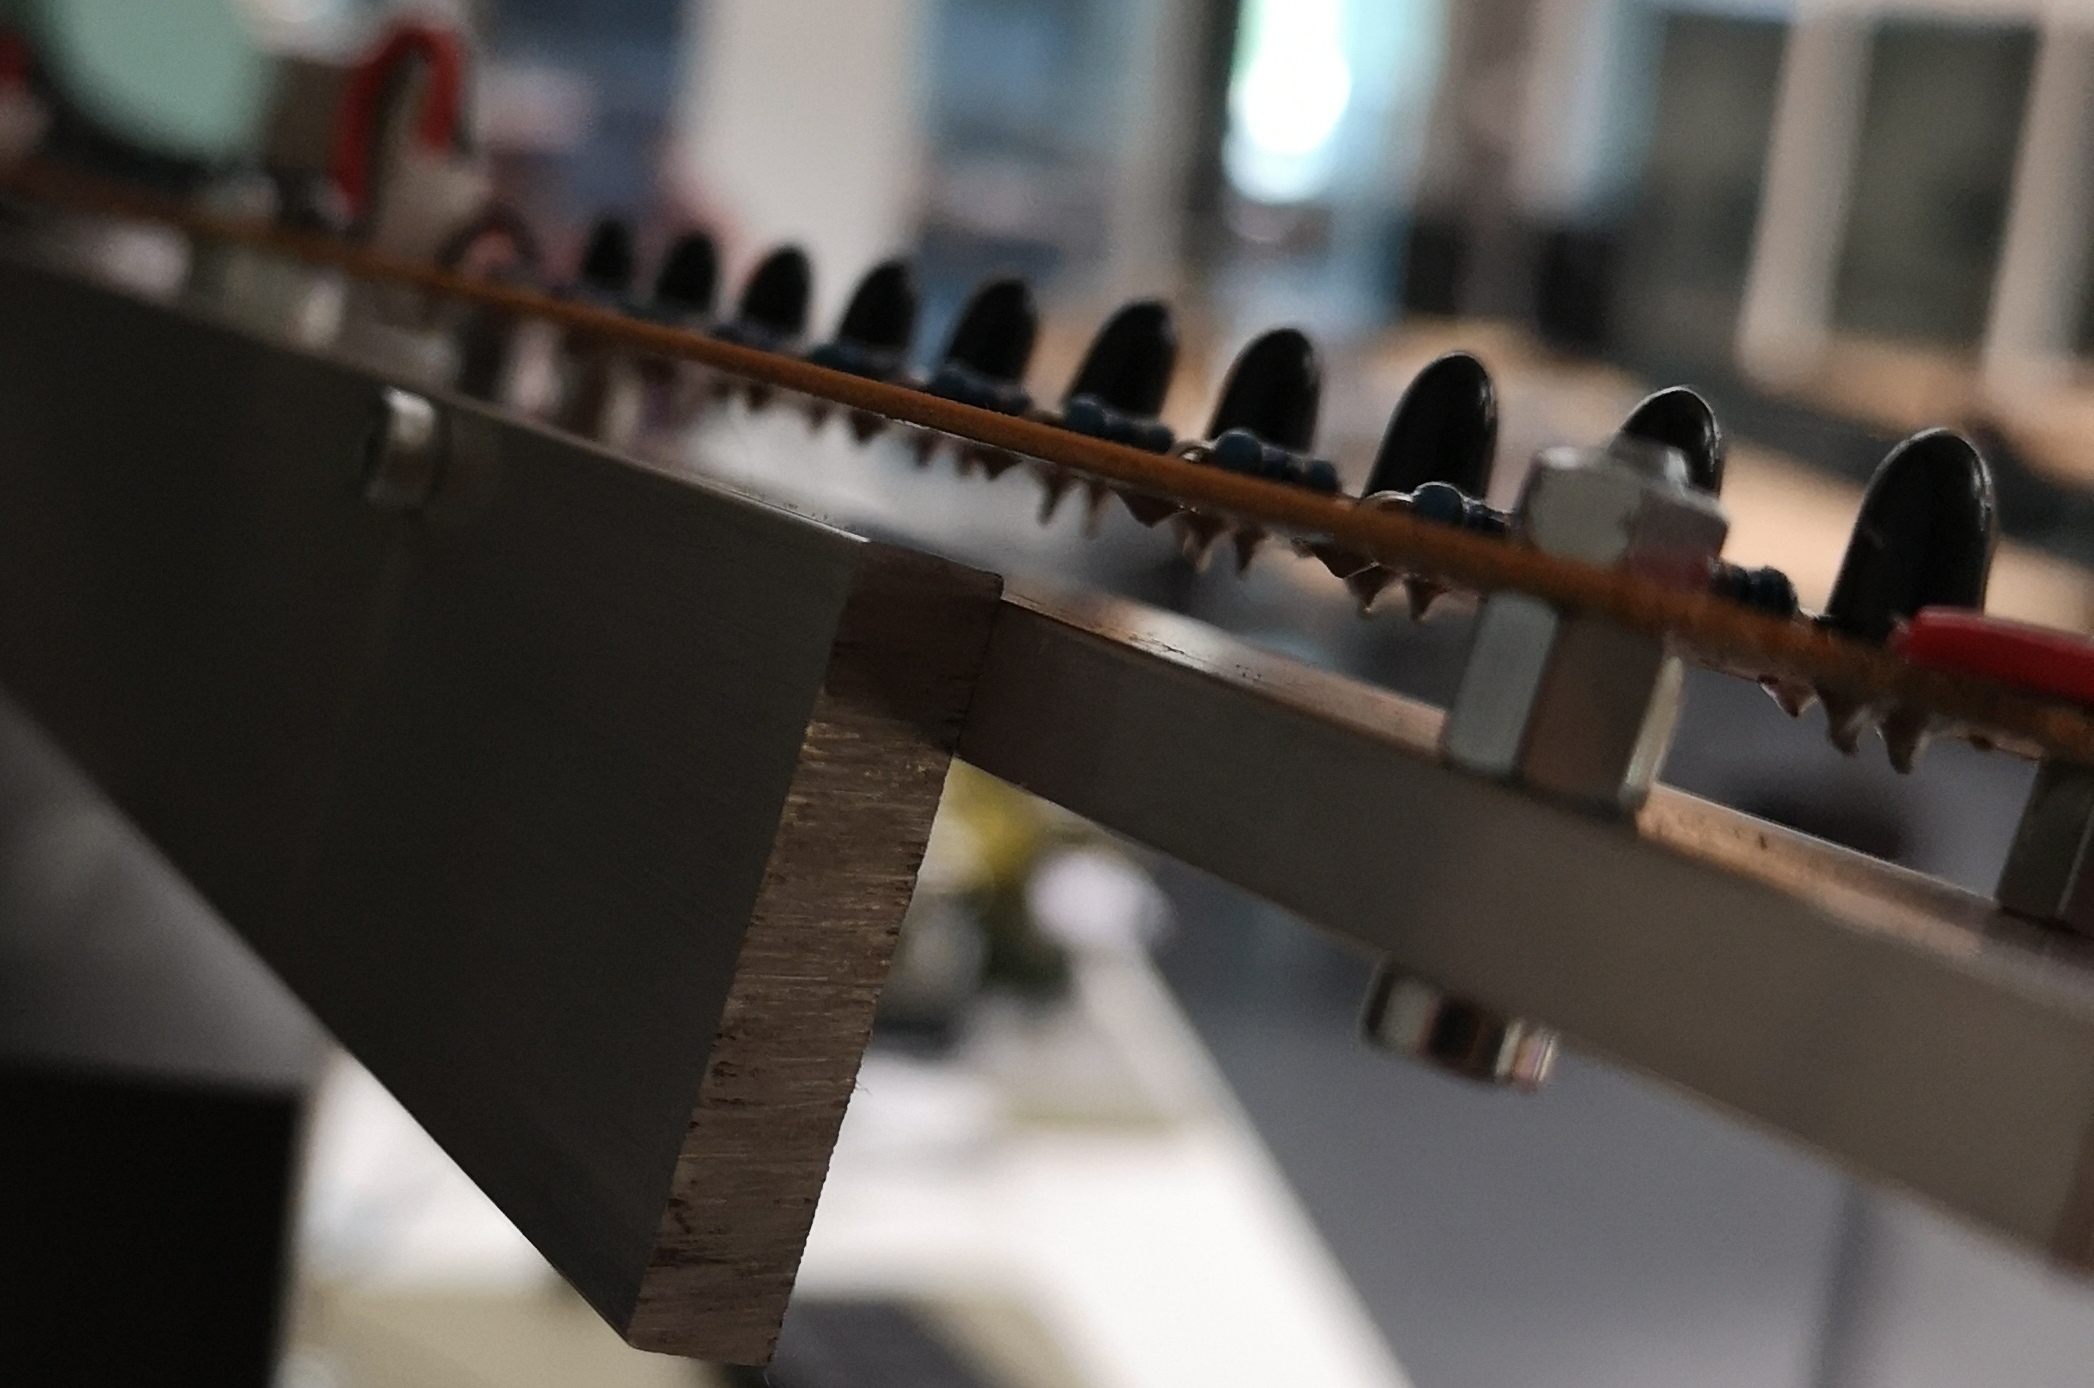
\includegraphics[height=4cm]{assets/figures/eclairage_cote.jpg}
    \caption{Assemblage - Angle anti-vibration}
\end{figure}

On notera qu'un second élément en aluminium a été vissé perpendiculairement au premier de manière à limiter les vibrations sur le rail d'éclairage.

\subsection{Capteur}
Le capteur et sont filtre seront placés dans un boitier étanche dont la façade est transparente. Pour être le plus centré possible, la caméra sera placée
le plus à gauche du boitier, plaquée contre l'extérieur.
\newpage
\section{Programme}
\subsection{Librairies}
Le fonctionnement du programme dépend de plusieurs librairies:
\begin{itemize}
    \item numpy
    \item time
    \item libcamera
    \item Picamera2
    \item openCV
    \item threading
    \item RPi.GPIO
\end{itemize}
Une partie des packages sont déjà présent par défaut dans l'OS utilisé, \underline{Raspbian Bullseye}, voici la liste des installations à faire:
\begin{itemize}
    \item sudo apt install python3-numpy
    \item sudo apt-get install libatlas-base-dev
    \item sudo apt install -y python3-picamera2
    \item sudo apt-get install python-opencv
    \item sudo apt-get install rpi.gpio
\end{itemize}
\subsection{Capture d'images de références}
\subsubsection{Paramètres}
Le traitement d'image permettant de mettre en valeur et détecter les hydrocarbures nécessite des images de références ayant été capturées dans des conditions précises et avec des paramètres de caméra maîtrisés.

Le programme de capture d'image de références fera plusieurs centaines de capture de la même zone à observer en faisant varier les paramètres suivants:
\begin{itemize}
    \item Temps d'exposition
    \item Gain analogique
    \item Balance des blancs
\end{itemize}

Le programme \underline{cap\_img\_ref.py} (annexe \ref{img_ref}) effectue les changements de paramètres et capture 3 images par configuration.
(la documentation de la caméra indique que l'ajustement des paramètres s'effectue en 3 frames maximum.)
Au terme des essais, la configuration idéal est la suivante:

\begin{table}[H]
    \begin{center}
        \caption{Table - Configuration caméra}
        \begin{tabular}{|c|c|}
            Elément              & Valeurs                 \\ \hline
            Temps d'exposition   & 1080 \si{\milli\second} \\
            Gain analogique      & 1.65                    \\
            Balance des blancs R & 0.9                     \\
            Balance des blancs B & 1.4                     \\
        \end{tabular}
    \end{center}
\end{table}

Cet configuration permet de capturer correctement les traces d'hydrocarbures de manière à ce qu'elle soit très visible lorsqu'on isole le premier layer de l'image.
\subsubsection{Résultats}
Une première séance de capture directement m'a permis d'effectuer des captures à l'aide du code mentionné précédemment: \underline{cap\_img\_ref.py}. Cependant, j'ai rencontré un problème, les captures sont floues, laissant penser que la mise au point est mal réglée.

\begin{figure}[H]
    \centering
    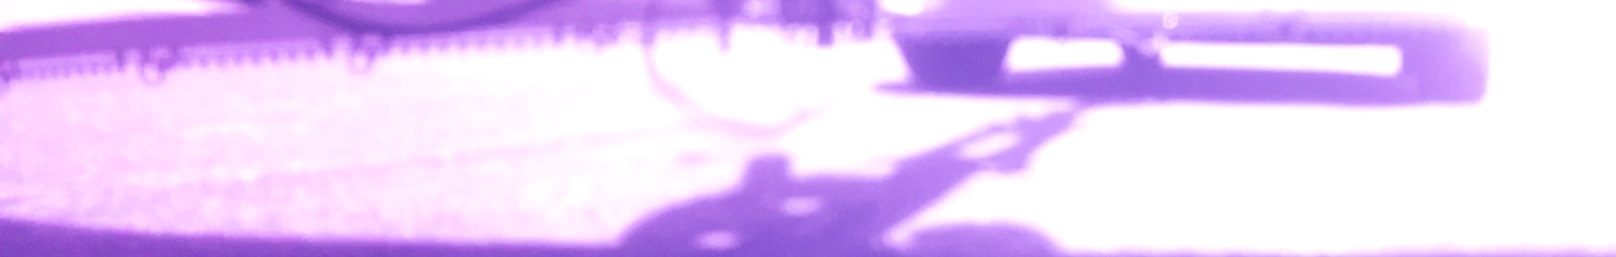
\includegraphics[height=2cm]{assets/figures/capture_floue.png}
    \caption{Capture - Image floue}
\end{figure}

La librairie Picamera2 \cite{picamera2} comprend une méthode qui règle la position de la lentille en fonction de la zone à observer pour la mise au point. La méthode a été testée en laboratoire et fonctionnait très bien. Durant la séance de capture,
la mise au point était définie pour observer les éléments à 90 \si{\centi\meter} de l'objectif.

En reproduisant le problème en laboratoire, j'ai compris que c'est la vitre de protection qui gène, en la retirant ou simplement en mettant de la distance entre la vitre et l'objectif, l'image redevient nette.

J'estime donc que plusieurs solutions qui s'offrent à moi.
\begin{enumerate}
    \item Revoir le placement de la caméra dans le boitier de manière à ne pas coller l'objectif à la vitre.
    \item Jouer avec le paramètre du focus et trouver une valeur pour laquelle l'image est nette derrière la vitre.
    \item Faire un trou de la taille de l'objectif dans la vitre du boitier.
\end{enumerate}

La première solution est la plus facilement et rapidement réalisable. J'ai ajouté un jeu de vis et de boulons dans les trous déjà existant sur le PCB de la caméra.
Ils servent ainsi de butées lorsque le tout est plaqué contre la vitre du boitier.

Cette solution permet d'avoir des images nets ressemblant à ceci:
\begin{figure}[H]
    \centering
    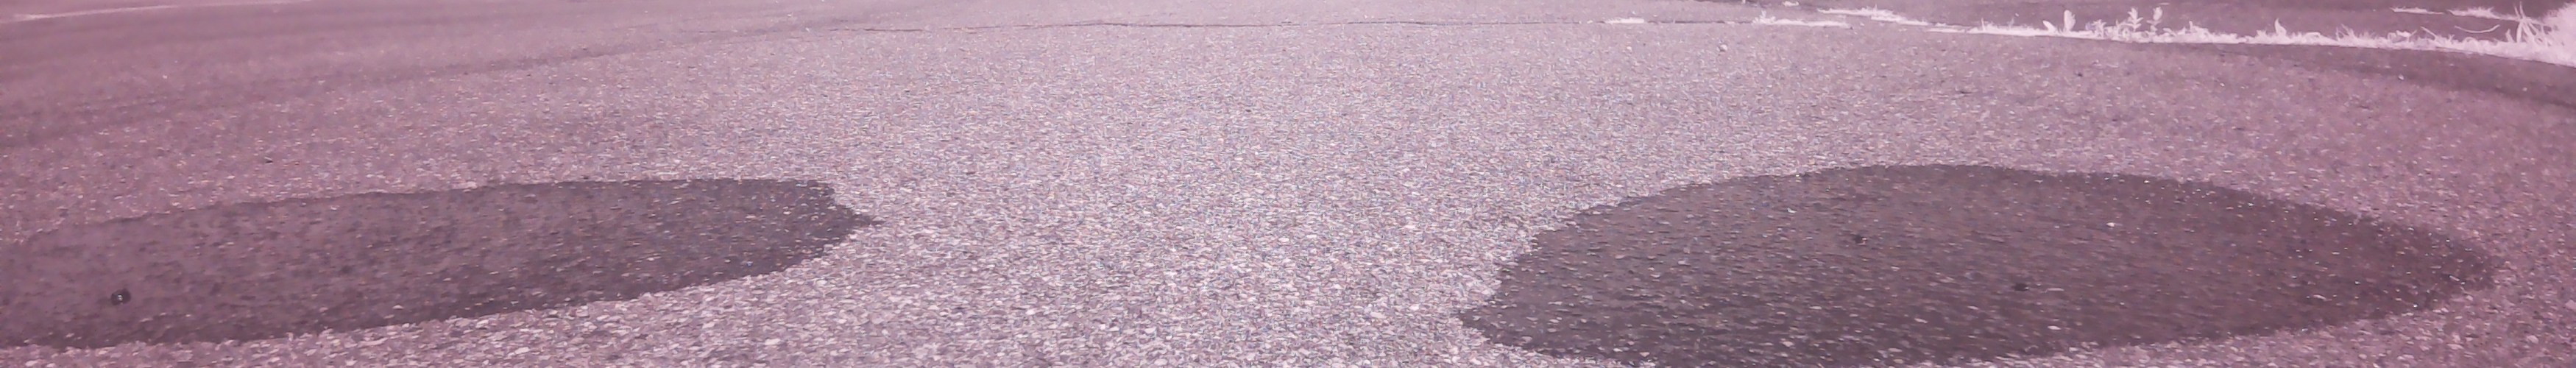
\includegraphics[width=13cm]{assets/figures/oil_test.png}
    \caption{Détection - Image de référence}
\end{figure}
\newpage

\subsection{Traitement de l'image}
\subsubsection{Structure de la partie traitement}
\begin{figure}[H]
    \centering
    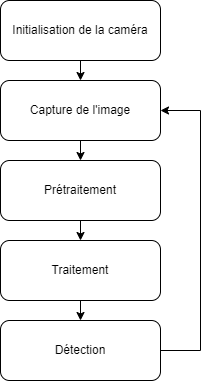
\includegraphics[height=8cm]{assets/figures/diagramme_traitement.png}
    \caption{Détection - Diagramme du traitement}
\end{figure}

Le programme principal (annexe \ref{main}) consiste en l'appel successif de fonction provenant de la librairie du fichier \underline{detection\_lib.py} (annexe \ref{libraire_det}).
Les fonctions correspondantes au diagramme sont respectivement:
\begin{itemize}
    \item init\_camera(resolution, distance), fonction qui configure et démarre la caméra.
    \item capture(camera), fonction qui effectue une capture et renvoie l'image.
    \item pretreatment(image, layer, threshold), fonction qui binarise l'image, par rapport au threshold et au layer souhaité.
    \item treatment(image\_bin), fonction qui effectue la mise en avant des tâches d'hydrocarbures. Les fonctions d'openCV sont utilisées pour effectuer un opening sur l'image binarisée.
    \item zone\_detection(line), fonction qui retourne le taux d'ouverture requis pour chaque vérin. Une ligne de pixel est donnée en paramètre. L'emplacement des zones à traiter sont déterminés et l'ouverture est retournée en fonction de la largeur des traces dans chaque section.
\end{itemize}

\subsection{Aperçu du traitement}
Une fois le prétraitement et le traitement effectués, l'image résultante est la suivante:

\begin{figure}[H]
    \centering
    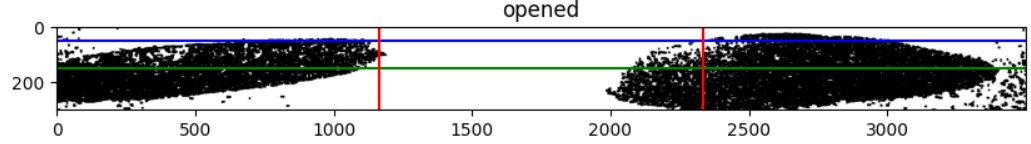
\includegraphics[width=13cm]{assets/figures/traitement1.PNG}
    \caption{Détection - Image traitée, en rouge, la séparation des sections}
\end{figure}

Puis en passant une ligne de pixel à \underline{zone\_detection()}, par exemple les lignes verte, bleue et violette de l'image précédente, la fonction
nous retourne le pourcentage d'ouverture de chaque section. L'ouverture retournée correspond au rapport entre la largeur de la tâche et de la section.

\begin{table}[H]
    \begin{center}
        \caption{Table - Détection, ouverture des vérins}
        \begin{tabular}{|c|c|c|c|}
            Ligne    & Gauche & Centre & Droite \\ \hline
            Bleue    & 24 \%  & 0 \%   & 42 \%  \\
            Verte    & 85 \%  & 14 \%  & 84 \%  \\
            Violette & 0 \%   & 18 \%  & 41 \%  \\
        \end{tabular}
    \end{center}
\end{table}

\subsection{Temps d'exécution}
Le temps d'exécution moyen du code présenté a été mesuré.
\begin{table}[H]
    \begin{center}
        \caption{Table - Temps d'exécution moyen}
        \begin{tabular}{|c|c|}
            Etapes             & Temps moyens [ms] \\ \hline
            Capture            & 88.922            \\
            Traitement         & 131.21            \\
            Calcul d'ouverture & 0.275             \\ \hline
            Total              & 220.407           \\
        \end{tabular}
    \end{center}
\end{table}

Si le semoir se déplace à une vitesse de 5 [km/h] (1.388 [m/s]), il est possible de connaitre la distance entre deux captures et traitement: \(d = v * t = 1.388 * 0.220407 = 0.30612 [m] \), c'est environ une image toute les 30 [cm].

La capture a un temps fix, je ne pense pas qu'il est possible de l'abaisser. Il est par contre certainement possible de réduire le temps de traitement, soit en optimisant l'algorithme utilisé, soit éventuellement en travaillant en parallèle de la capture.